% =====================================================================
%  BreathNote: Smart Incentive Spirometer -- Final Project Report
%  Same style as the idea-submission concept document (proposal.tex).
%
%  Compile with pdfLaTeX (run twice so the contents and page numbers settle):
%      pdflatex report.tex
%      pdflatex report.tex
% =====================================================================
\documentclass[12pt,a4paper]{article}

% ---------- Page layout ----------------------------------------------
\usepackage[a4paper, margin=2.5cm]{geometry}

% ---------- Fonts ----------------------------------------------------
\usepackage[T1]{fontenc}
\usepackage{textcomp}
\usepackage{tgtermes}                   % Times-style serif for all text
\usepackage{microtype}
\linespread{1.03}

\newcommand{\rupee}{Rs.\,}              % currency prefix used in the text
\newcommand{\Sah}{Sa\ensuremath{'}}     % upper (high) Sa

% ---------- Paragraphs, lists, headings ------------------------------
\setlength{\parindent}{0pt}
\setlength{\parskip}{6pt}
\widowpenalty=10000
\clubpenalty=10000

\usepackage{enumitem}
\setlist{itemsep=2pt, topsep=4pt, parsep=0pt, leftmargin=1.5em}

\usepackage{titlesec}
\titleformat{\section}{\normalfont\large\bfseries}{\thesection.}{0.5em}{}
\titlespacing*{\section}{0pt}{16pt}{6pt}
\titleformat{\subsection}{\normalfont\normalsize\bfseries}{\thesubsection}{0.5em}{}
\titlespacing*{\subsection}{0pt}{10pt}{4pt}
\titleformat{\subsubsection}{\normalfont\normalsize\bfseries\itshape}{\thesubsubsection}{0.5em}{}
\titlespacing*{\subsubsection}{0pt}{8pt}{3pt}
\setcounter{secnumdepth}{3}
\setcounter{tocdepth}{2}
\usepackage{multicol}
\usepackage[titles]{tocloft}
\setlength{\cftbeforesecskip}{1.5pt}
\setlength{\cftbeforesubsecskip}{0pt}
\setlength{\cftsubsecnumwidth}{2.6em}
\setlength{\cftsubsecindent}{1.2em}
\renewcommand{\cftdotsep}{2}
\cftsetrmarg{2.55em plus 1fil}
\renewcommand{\cftsecfont}{\bfseries\small}
\renewcommand{\cftsecpagefont}{\bfseries\small}
\renewcommand{\cftsubsecfont}{\small}
\renewcommand{\cftsubsecpagefont}{\small}

% ---------- Tables and figures ---------------------------------------
\usepackage{array, booktabs, tabularx, longtable, multirow}
\renewcommand{\arraystretch}{1.2}
\newcolumntype{L}{>{\raggedright\arraybackslash\hyphenpenalty=10000}X}
\newcolumntype{P}[1]{>{\raggedright\arraybackslash\hyphenpenalty=10000}p{#1}}

\usepackage{amsmath}
\usepackage{graphicx}
\usepackage{float}
\usepackage{placeins}                      % [H] keeps a table under its heading
\usepackage{needspace}                  % keeps a heading with its table
\usepackage{caption}
\usepackage{subcaption}
\captionsetup{font=small, labelfont=bf, labelsep=colon, skip=6pt}
\captionsetup[table]{position=top}

\usepackage{tikz}
\usetikzlibrary{positioning, arrows.meta, calc, shapes.geometric, fit, backgrounds}
\usepackage{pgfplots}
\pgfplotsset{compat=1.16}

% ---------- Page numbers ---------------------------------------------
\usepackage{fancyhdr, lastpage}
\pagestyle{fancy}
\fancyhf{}
\fancyfoot[C]{\small Page \thepage{} of \pageref{LastPage}}
\renewcommand{\headrulewidth}{0pt}
\fancypagestyle{plain}{\fancyhf{}\fancyfoot[C]{\small Page \thepage{} of \pageref{LastPage}}}

% ---------- Links (printed in black) ---------------------------------
\usepackage{hyperref}
\hypersetup{
  colorlinks=true, urlcolor=blue, linkcolor=black, citecolor=black,
  pdftitle={BreathNote: A Smart Incentive Spirometer with Breath-Driven Music Feedback -- Final Report},
  pdfauthor={Ande Karthik, Kalluri Roshan Lal, Pasumarthy Deepak}}
\urlstyle{same}

% ---------- Project details (edit here) ------------------------------
\newcommand{\githuburl}{https://github.com/Roshan-o/Spirometer}
\newcommand{\videourl}{https://drive.google.com/file/d/18UdDUZlwO37Ve3utC2zd_bIKU9YbzDy5/view}
\newcommand{\driveurl}{https://drive.google.com/drive/folders/1bPdsBMErJisqiP8W3hTLAdX8OIbYA5W-?usp=sharing}
\newcommand{\sevaurl}{https://drive.google.com/drive/folders/1aHvxULoR30UtWy43ls5HY10PJA5bWtyK?usp=sharing}
\newcommand{\figmaurl}{https://www.figma.com/design/ZbQEwTaLI2R1L9XhwzSnIZ/Music?t=hc86C48bEpRClTkQ-1}

% A small framed note used for "In simple words" summaries.
\newcommand{\simple}[1]{%
  \par\smallskip\noindent
  \fbox{\parbox{\dimexpr\linewidth-2\fboxsep-2\fboxrule\relax}{\small\textbf{In simple words:} #1}}%
  \par\smallskip}

% =====================================================================
\begin{document}
\thispagestyle{plain}

% ---------- Title block ----------------------------------------------
\begin{center}
  {\LARGE\bfseries BreathNote\par}
  \vspace{6pt}
  {\Large A Smart Incentive Spirometer with\\ Breath-Driven Music Feedback\par}
  \vspace{10pt}
  {\large Final Project Report\par}
  \vspace{18pt}
  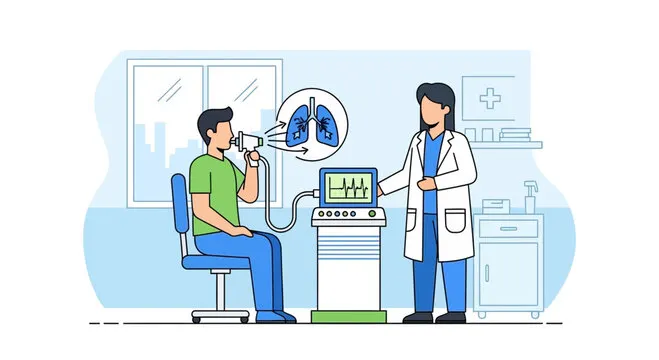
\includegraphics[width=0.85\linewidth]{figures/cover.png}\par
  \vspace{18pt}
  {\normalsize
  \begin{tabular}{@{}c@{\hspace{2.2em}}c@{\hspace{2.2em}}c@{}}
    Ande Karthik & Kalluri Roshan Lal & Pasumarthy Deepak \\
    2023102009   & 2023102010         & 2023101109
  \end{tabular}\\[8pt]
  International Institute of Information Technology, Hyderabad\\[2pt]
  November 2026\par}
\end{center}
\vspace{4pt}

\begin{center}
\small
\begin{tabular}{@{}r l@{}}
  \textbf{Video demo:}  & \href{\videourl}{Google Drive video} \\
  \textbf{Source code:} & \url{\githuburl} \\
  \textbf{Figma design:} & \href{\figmaurl}{Figma file ``Music''} \\
  \textbf{Sprint documents:} & \href{\driveurl}{Google Drive folder} \\
  \textbf{Idea submission:} & \href{\sevaurl}{Seva First Innovation Challenge submissions}
\end{tabular}
\end{center}

\newpage
\section*{Contents}
{\setlength{\parskip}{0pt}\linespread{0.95}\selectfont\hyphenpenalty=10000\exhyphenpenalty=10000
\makeatletter\@starttoc{toc}\makeatother}
\newpage

% =====================================================================
\section*{Abstract}
\addcontentsline{toc}{section}{Abstract}

After surgery, or while recovering from a lung illness, patients are asked to use an \textbf{incentive spirometer} many times a day to keep their lungs healthy. The exercise is repetitive and boring, the device gives no reward, and it keeps no track of how the user is performing. So many patients skip it, and the doctor cannot see whether they are improving.

\textbf{BreathNote} turns the ordinary incentive spirometer into a \textbf{digital spirometer} with \textbf{music integration} and \textbf{progress tracking}. A low-cost sensor added to the device measures each breath, and the breath itself plays calming music that grows richer as the patient breathes deeper and longer. This makes the exercise engaging and rewards the correct technique. Every session is recorded and shown on a personal dashboard, reminders prompt the patient to practise on time, and a progress report can be shared with the doctor.

A working, low-cost prototype has been built and tested end to end, and the idea was submitted to the Seva First Innovation Challenge on behalf of IIIT Hyderabad. The next step is a hospital pilot with real patients.

% =====================================================================
\section{What is a Spirometer?}
\label{sec:what}

A \textbf{spirometer} is a device that measures breathing. The word comes from the Latin \emph{spirare}, ``to breathe'', and the Greek \emph{metron}, ``measure''. There are two very different kinds of spirometer, and it is important not to mix them up.

\begin{enumerate}
  \item \textbf{Diagnostic spirometer.} This is a medical test machine used in hospitals and clinics. The patient takes the deepest breath possible and blows out as hard and as fast as possible into it. The machine measures \emph{how much} air comes out and \emph{how fast}. Doctors use these numbers to diagnose and monitor diseases such as asthma and COPD (chronic obstructive pulmonary disease). The two most important numbers are:
  \begin{itemize}
    \item \textbf{FVC} (Forced Vital Capacity): the total amount of air a person can blow out after a full breath in.
    \item \textbf{FEV\textsubscript{1}} (Forced Expiratory Volume in 1 second): how much of that air comes out in the first second.
  \end{itemize}
  \item \textbf{Incentive spirometer.} This is a simple, cheap, hand-held \emph{exercise} device. It does not diagnose anything. It encourages (gives an ``incentive'' to) the patient to take slow, deep breaths, by showing a target that moves when the patient breathes in. It is mostly used after surgery and during recovery from lung illness.
\end{enumerate}

\textbf{BreathNote is built on the incentive spirometer}, and the most common type of incentive spirometer, the \textbf{3-ball spirometer} (Figure~\ref{fig:spiro}). It has:
\begin{itemize}
  \item a \textbf{mouthpiece} that the patient seals with the lips;
  \item a flexible \textbf{tube} that connects the mouthpiece to the body of the device;
  \item a clear plastic \textbf{body with three chambers}, each holding one light plastic \textbf{ball}. The three balls need different amounts of breathing effort to lift. On common models the chambers are marked about 600, 900 and 1,200\,mL per second of airflow.
\end{itemize}

\begin{figure}[H]
  \centering
  \begin{subfigure}[b]{0.36\linewidth}
    \centering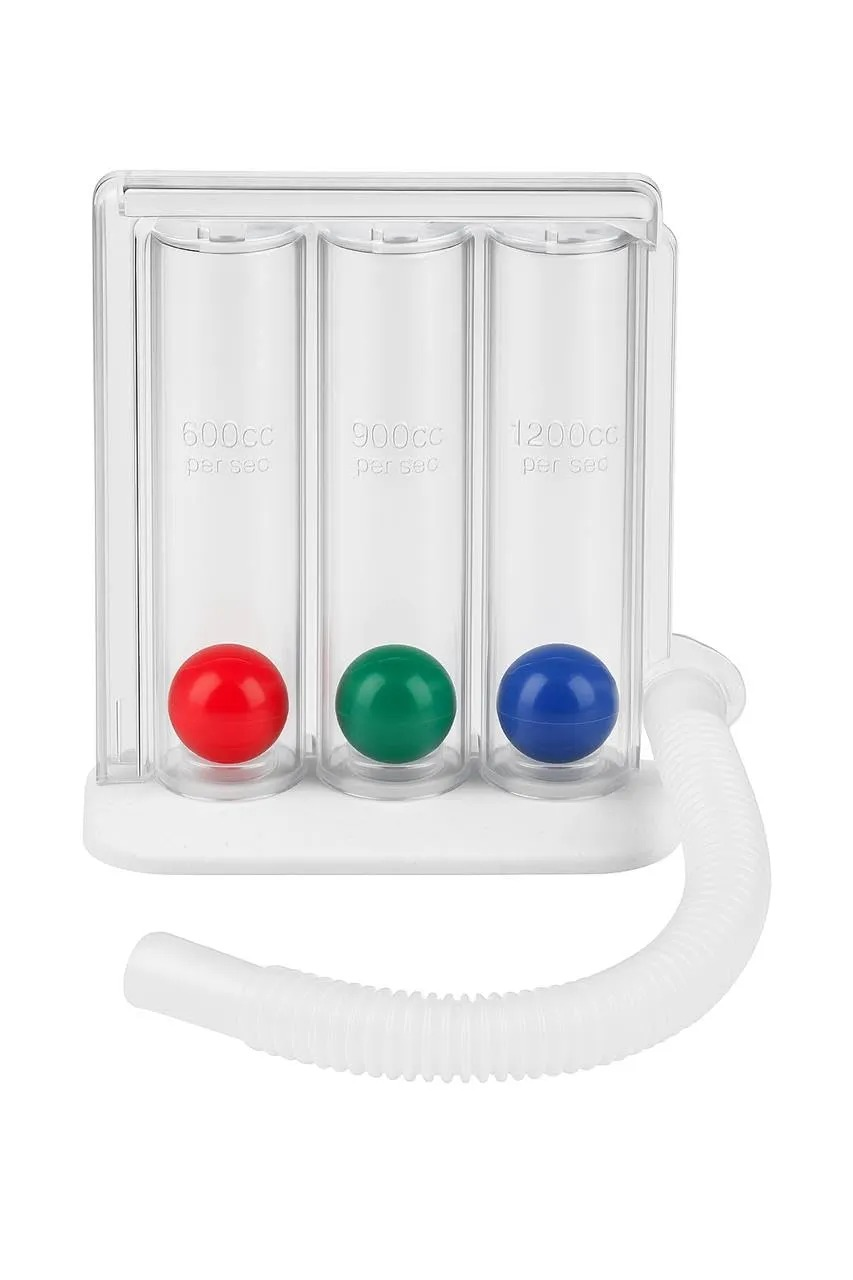
\includegraphics[height=4.6cm]{figures/spirometer.png}
    \caption{The 3-ball incentive spirometer.}
  \end{subfigure}\hspace{1.5em}
  \begin{subfigure}[b]{0.46\linewidth}
    \centering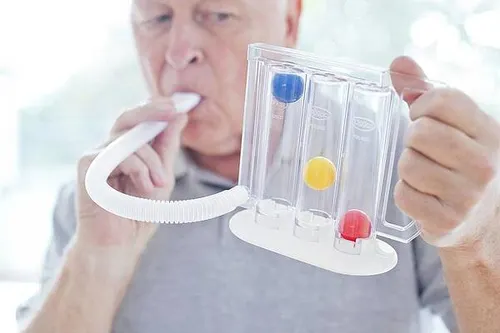
\includegraphics[height=4.6cm]{figures/patient_using.png}
    \caption{A patient using it: slow, deep breath in.}
  \end{subfigure}
  \caption{The conventional 3-ball incentive spirometer, which BreathNote upgrades.}
  \label{fig:spiro}
\end{figure}

% =====================================================================
\section{History of the Spirometer}
\label{sec:history}

People have tried to measure breathing for almost two thousand years. The story moves from simple bags and jars of water, to the first true spirometer in 1846, to electronic devices, and finally to the ``smart'' connected devices of today. BreathNote belongs to this last step.

\subsection{Early ideas (2nd century -- 1700s)}
\begin{itemize}
  \item \textbf{Galen (about 150 AD)}, a Greek physician in Rome, did one of the first breathing experiments. A boy breathed in and out of an animal bladder, and Galen noticed that the volume of air did not change. This was the first attempt to think about the ``amount'' of air in a breath.
  \item \textbf{Giovanni Borelli (1679)}, an Italian scientist, measured the volume of air taken in during a single breath by drawing air through a tube from a cylinder.
  \item \textbf{James Jurin (1718)} blew into a bladder and measured the volume of air by how much water it pushed out. He estimated that a normal breath is about 650\,mL and a deep breath about 3.6\,L, which is close to modern values.
\end{itemize}

\subsection{The first real spirometer (1800s)}
\begin{itemize}
  \item \textbf{Edward Kentish (1813)} built the ``pulmometer'', a graduated bell jar standing upside down in water. The patient breathed into it and the bell rose.
  \item \textbf{John Hutchinson (1846)}, a London surgeon, invented the \textbf{water spirometer} and gave it its name. A light bell floated in water and rose when the person blew into it; a scale showed the volume. Hutchinson measured more than 4,000 people and defined the \textbf{vital capacity}: the largest amount of air a person can breathe out after the deepest breath in. He showed that vital capacity depends on height and falls with age and disease. This is the birth of spirometry.
\end{itemize}

\subsection{Speed of breathing and standardisation (1900s)}
\begin{itemize}
  \item \textbf{Tiffeneau and Pinelli (1947)} in France added \emph{time}: how much air comes out in the first second. This became FEV\textsubscript{1}, still the most important lung function number today.
  \item \textbf{Gaensler (1951)} introduced the ratio FEV\textsubscript{1}/FVC to separate blocked airways (as in asthma and COPD) from stiff lungs.
  \item \textbf{Wright (1959)} invented the peak flow meter, a small device to measure how fast a person can blow out.
  \item \textbf{1970s:} electronic spirometers with flow sensors (pneumotachographs) and computers replaced water bells.
  \item \textbf{1979 onwards:} the American Thoracic Society, and later the ATS and European Respiratory Society together (2005, updated 2019), published standards for how spirometry must be done and how accurate devices must be.
\end{itemize}

\subsection{The incentive spirometer (1970s)}
In the early 1970s, \textbf{Robert Bartlett and colleagues} studied why patients develop lung complications after surgery. They showed that pain makes patients take small, shallow breaths, so parts of the lung collapse. They proposed that patients should regularly take a \emph{sustained maximal inspiration}: a slow, deep breath held at the top. To make patients do this on their own, a simple device with a visible target was created: the \textbf{incentive spirometer}. Two designs became common:
\begin{itemize}
  \item \textbf{Flow-oriented} devices, such as the 3-ball spirometer, where balls rise with the airflow.
  \item \textbf{Volume-oriented} devices, where a piston rises to show the volume breathed in.
\end{itemize}
The 3-ball device is cheap, needs no power and is now used in hospitals all over the world, including India.

\subsection{Digital and smart spirometers (2000s -- today)}
\begin{itemize}
  \item Portable electronic spirometers and USB spirometers brought lung testing to clinics and homes.
  \item \textbf{SpiroSmart (2012)} showed that a smartphone microphone can estimate lung function.
  \item Research groups built \textbf{electronic incentive spirometers} that add a flow sensor to a 3-ball device \cite{silva}, and \textbf{frugal Arduino spirometers} for low-resource settings \cite{wallace}.
  \item A \textbf{reminder device} attached to the incentive spirometer (SpiroTimer) was tested in a randomised trial after heart bypass surgery; reminders increased how often patients used the spirometer \cite{eltorai2019}.
\end{itemize}

\begin{figure}[H]
\centering
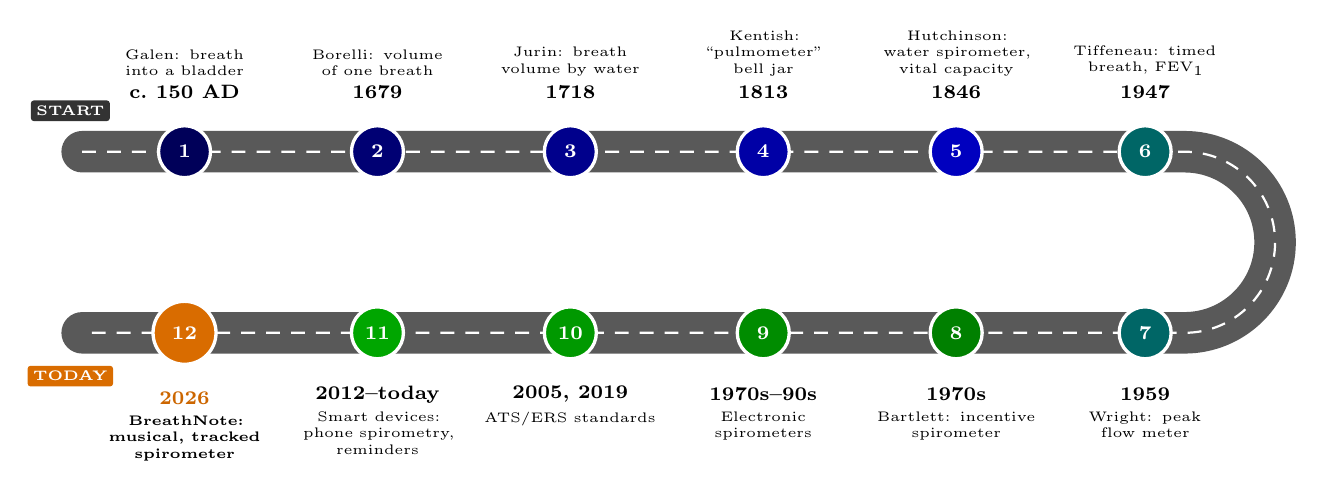
\begin{tikzpicture}[
    cp/.style={circle, draw=white, line width=1.2pt, minimum size=6.6mm, inner sep=0pt,
               font=\scriptsize\bfseries\color{white}},
    yr/.style={font=\scriptsize\bfseries, align=center},
    txt/.style={font=\tiny, align=center, text width=2.2cm, inner sep=1pt,
               execute at begin node={\hyphenpenalty=10000 \exhyphenpenalty=10000 }}]
  % ---- the road: left to right, U-turn, right to left ----
  \def\roadpath{(-0.4,3.6) -- (13.6,3.6) arc[start angle=90, end angle=-90, radius=1.15] -- (-0.4,1.3)}
  \draw[line width=15pt, black!65, line cap=round] \roadpath;
  \draw[line width=0.8pt, white, dash pattern=on 5pt off 4pt] \roadpath;
  % start and finish flags
  \node[font=\tiny\bfseries, fill=black!80, text=white, rounded corners=1pt, inner sep=2pt] at (-0.55,4.12) {START};
  \node[font=\tiny\bfseries, fill=orange!85!black, text=white, rounded corners=1pt, inner sep=2pt] at (-0.55,0.75) {TODAY};
  % ---- row 1 (past), labels above ----
  \foreach \i/\x/\c/\y/\t in {
      1/0.9/blue!35!black/c.\ 150 AD/{Galen: breath into a bladder},
      2/3.35/blue!45!black/1679/{Borelli: volume of one breath},
      3/5.8/blue!55!black/1718/{Jurin: breath volume by water},
      4/8.25/blue!65!black/1813/{Kentish: ``pulmometer'' bell jar},
      5/10.7/blue!75!black/1846/{Hutchinson: water spirometer, vital capacity},
      6/13.1/teal!80!black/1947/{Tiffeneau: timed breath, FEV\textsubscript{1}}}{
    \node[cp, fill=\c] at (\x,3.6) {\i};
    \node[yr] at (\x,4.36) {\y};
    \node[txt, anchor=south] at (\x,4.52) {\t};
  }
  % ---- row 2 (modern), labels below ----
  \foreach \i/\x/\c/\y/\t in {
      7/13.1/teal!80!black/1959/{Wright: peak flow meter},
      8/10.7/green!50!black/1970s/{Bartlett: incentive spirometer},
      9/8.25/green!55!black/1970s--90s/{Electronic spirometers},
      10/5.8/green!60!black/{2005, 2019}/{ATS/ERS standards},
      11/3.35/green!65!black/2012--today/{Smart devices: phone spirometry, reminders}}{
    \node[cp, fill=\c] at (\x,1.3) {\i};
    \node[yr] at (\x,0.52) {\y};
    \node[txt, anchor=north] at (\x,0.34) {\t};
  }
  % ---- final checkpoint: BreathNote ----
  \node[cp, fill=orange!85!black, minimum size=8mm, font=\scriptsize\bfseries\color{white}] at (0.9,1.3) {12};
  \node[yr, text=orange!80!black] at (0.9,0.47) {2026};
  \node[txt, anchor=north, font=\tiny\bfseries] at (0.9,0.29) {BreathNote: musical, tracked spirometer};
\end{tikzpicture}
\caption{The road of the spirometer, from the first breathing experiments to BreathNote.}
\label{fig:road}
\end{figure}

% =====================================================================
\section{Working Principle of the Spirometer}
\label{sec:principle}

\subsection{How breathing works}
When we breathe in, the \textbf{diaphragm} (a dome-shaped muscle under the lungs) contracts and moves down, and the ribs move up and out. The chest becomes bigger, so the pressure inside the lungs falls slightly below the pressure of the room air. Air always moves from high pressure to low pressure, so air flows in through the mouth. When we breathe out, the muscles relax, the chest becomes smaller, the pressure inside rises, and air flows out.

After surgery, pain and medicines make patients breathe in small, shallow breaths. The bottom parts of the lungs do not open fully. The tiny air sacs (alveoli) can collapse; this is called \textbf{atelectasis}. Mucus collects, and infections such as \textbf{pneumonia} can start. A slow, deep breath held for a few seconds opens these air sacs again.

\subsection{How a 3-ball incentive spirometer works}
\begin{enumerate}
  \item The patient places the mouthpiece in the mouth and \textbf{inhales slowly and deeply}.
  \item During inhalation, the \textbf{diaphragm moves downward}, creating low pressure inside the lungs.
  \item Because of this low pressure, \textbf{air flows from the room through the spirometer into the lungs}.
  \item The moving air passes through the \textbf{three chambers} and creates an upward airflow.
  \item The \textbf{airflow lifts the plastic balls}. Each ball rises when the airflow is strong enough to overcome its weight.
  \item The three balls are calibrated for \textbf{different airflow levels} (approximately 600, 900 and 1,200\,mL/s). More airflow causes more balls to rise.
  \item The patient \textbf{holds the raised ball(s) for 3--5 seconds} and then exhales normally.
\end{enumerate}

\begin{figure}[H]
\centering
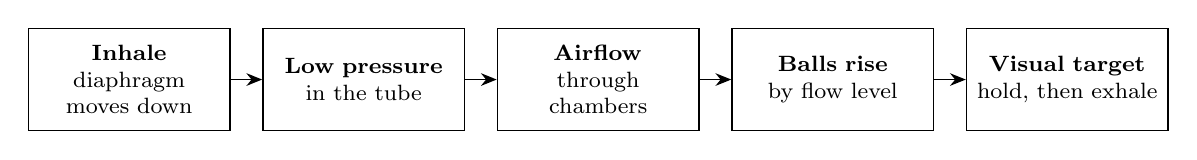
\begin{tikzpicture}[
    node distance=4mm,
    box/.style={draw=black, fill=white, line width=0.5pt, align=center,
                text width=2.35cm, minimum height=13mm, inner sep=3pt, font=\footnotesize},
    arr/.style={-{Stealth[length=2mm, width=1.6mm]}, line width=0.6pt}]
  \node[box] (a) {\textbf{Inhale}\\ diaphragm moves down};
  \node[box, right=of a] (b) {\textbf{Low pressure}\\ in the tube};
  \node[box, right=of b] (c) {\textbf{Airflow}\\ through chambers};
  \node[box, right=of c] (d) {\textbf{Balls rise}\\ by flow level};
  \node[box, right=of d] (e) {\textbf{Visual target}\\ hold, then exhale};
  \draw[arr] (a)--(b); \draw[arr] (b)--(c); \draw[arr] (c)--(d); \draw[arr] (d)--(e);
\end{tikzpicture}
\caption{Working principle of a 3-ball incentive spirometer.}
\label{fig:principle}
\end{figure}

\textbf{Note:}
\begin{itemize}
  \item Posture, mouthpiece seal, technique, pain and the illness itself all change how high the balls go.
  \item \textbf{There is no single ``normal'' reading.} The right target depends on the patient's age, sex, medical conditions and the reason for using the device. The doctor uses these to set the patient's goal \cite{verywell}.
\end{itemize}

% =====================================================================
\section{Who Can Use This Spirometer and Why?}
\label{sec:users}

The incentive spirometer, and therefore BreathNote, is useful for many groups of people. Figures~\ref{fig:users-who} and~\ref{fig:lung-exerciser} show the main users, and the list below explains why each group uses it.

\textbf{Patients:}
\begin{itemize}
  \item \textbf{Patients with COPD, asthma, post-COVID weakness:} Practise slow, deep breathing and keep the lungs open.
  \item \textbf{Patients with emphysema, chronic bronchitis or bronchiectasis:} Help manage these long-term lung conditions \cite{verywell}.
  \item \textbf{Patients recovering from severe pneumonia:} Re-open the lungs and clear mucus.
  \item \textbf{Patients with cystic fibrosis, and children with cerebral palsy:} Keep the airways clear and the lungs active.
  \item \textbf{Patients with restrictive lung disease:} Help the lungs expand more fully.
  \item \textbf{Patients with neuromuscular disease or spinal cord injury:} These weaken the breathing muscles; regular deep breaths keep the lungs working.
\end{itemize}

\begin{figure}[H]
  \centering
  \begin{minipage}[t]{0.40\linewidth}
    \vspace{0pt}\centering
    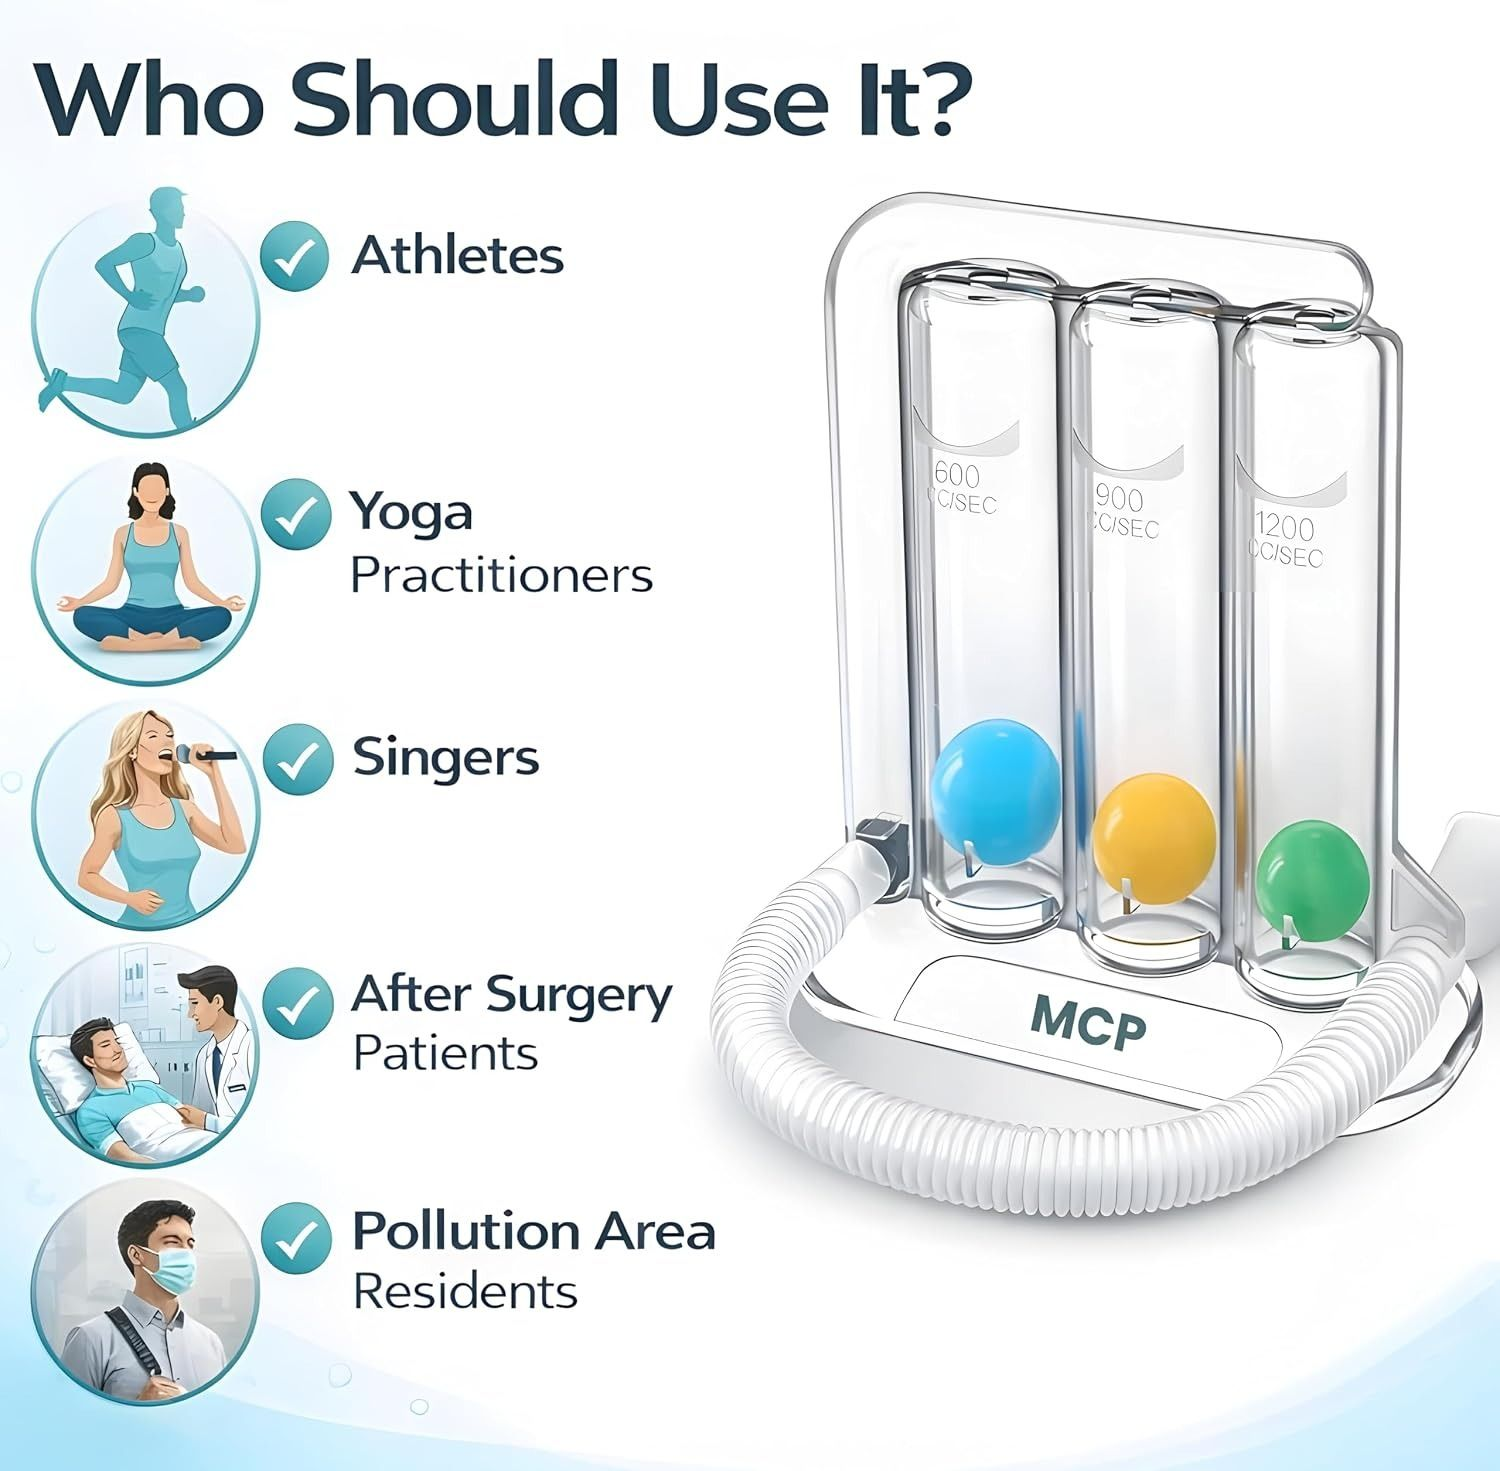
\includegraphics[height=4.6cm]{figures/who_uses.png}
    \captionof{figure}{People who can use it: athletes, yoga practitioners, singers, patients after surgery and people in polluted areas.}
    \label{fig:users-who}
  \end{minipage}\hfill
  \begin{minipage}[t]{0.56\linewidth}
    \vspace{0pt}\centering
    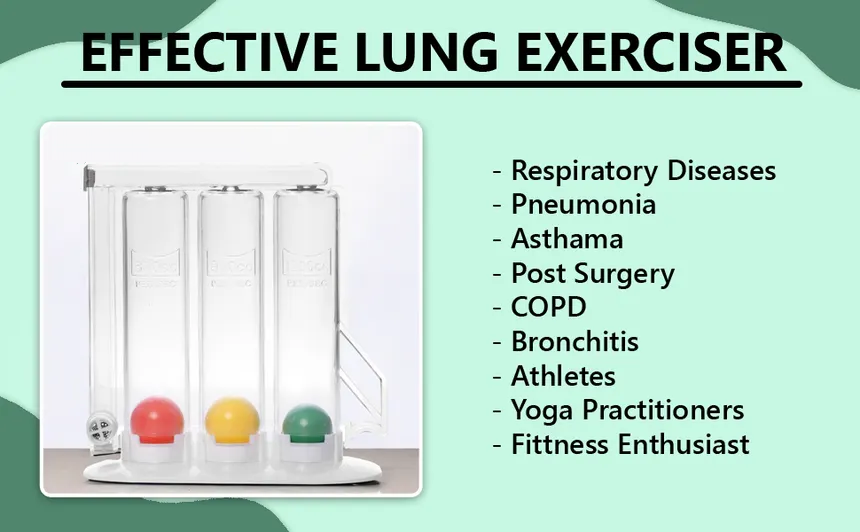
\includegraphics[height=4.6cm]{figures/lung_exerciser.png}
    \captionof{figure}{The 3-ball incentive spirometer as a lung exerciser for respiratory diseases, pneumonia, asthma, recovery after surgery, COPD, bronchitis, athletes, yoga practitioners and fitness enthusiasts.}
    \label{fig:lung-exerciser}
  \end{minipage}
\end{figure}

\textbf{Other users.} Healthy people can also use the device for breathing training (Table~\ref{tab:otherusers}).

\begin{table}[H]
\centering
\caption{Other users of the device and why they use it.}
\label{tab:otherusers}
\small
\begin{tabularx}{\linewidth}{@{}P{5.4cm} L@{}}
\toprule
\textbf{User} & \textbf{Why they use it} \\
\midrule
Athletes and fitness users (where appropriate) & Breathing control training \\
Singers, wind-instrument players and yoga practitioners & Breath control and sustained, steady exhalation and inhalation \\
People living in high-pollution areas & Regular breathing exercise for lung health (under medical advice) \\
\bottomrule
\end{tabularx}
\end{table}

\textbf{What the research says.} A 2019 study suggested that incentive spirometry after lung surgery reduces complications such as pneumonia, while other research suggests it may help less after weight-loss (bariatric) surgery \cite{verywell}.

% =====================================================================
\section{How to Use the Device Normally}
\label{sec:howto}

Every patient should follow the instructions of their own doctor or respiratory therapist. The general steps are \cite{cleveland, verywell}:
\begin{enumerate}
  \item \textbf{Sit upright} in a comfortable chair or on the edge of the bed.
  \item \textbf{Hold the device upright} with both hands. On a piston-type device, slide the goal indicator to the target level set by the doctor (a common starting mark is around 1,250 on the scale).
  \item \textbf{Breathe out normally.}
  \item \textbf{Seal your lips} tightly around the mouthpiece, and do not block it with your tongue.
  \item \textbf{Breathe in slowly and deeply} through the mouth. Watch the balls (or the piston) rise: try to raise the first ball, then the second, then the third. If the device has a flow indicator, keep it in the centre.
  \item \textbf{Hold the breath} for at least 3 seconds (3--5 seconds or more), keeping the balls up as long as you comfortably can. If you feel dizzy, take a break.
  \item \textbf{Take the mouthpiece out, breathe out normally and rest.} Cough to clear mucus if needed.
  \item On a piston-type device, \textbf{move the goal indicator to your best result} so you can try to beat it next time.
  \item \textbf{Repeat 10 to 12 times every hour while awake}, or as your doctor says. Do not be discouraged if you do not reach your goal at first; it improves with practice.
  \item After chest or abdominal surgery, \textbf{hold a pillow firmly against the wound} while breathing deeply and coughing; this makes it less painful.
\end{enumerate}

% =====================================================================
\section{Problem Statement}
\label{sec:problem}

The incentive spirometer is given to patients whose lungs do not expand fully, such as:
\begin{itemize}
  \item patients recovering from \textbf{chest, heart or abdominal surgery};
  \item patients with \textbf{respiratory illnesses} such as pneumonia, COPD or asthma;
  \item \textbf{elderly patients} and people on \textbf{long bed rest} or with limited movement;
  \item patients in \textbf{respiratory rehabilitation} and physiotherapy.
\end{itemize}
These patients are advised to use the device several times a day, typically \textbf{about 10 breaths every hour while awake} \cite{cleveland}, to improve lung expansion and support respiratory recovery. That is more than 100 breaths a day, for days or weeks. The medical idea is good, but the device has four problems:

\begin{enumerate}
  \item \textbf{The exercise is repetitive and boring.} The same action is repeated again and again with no change, so it is hard for patients to stay motivated. Many gradually lose interest and do the exercise inconsistently over time. Some do it wrongly (quick, sharp breaths instead of slow, deep ones) or stop using the device.
  \item \textbf{The device gives no motivation.} It provides only immediate visual feedback through mechanical ball movement. There is no sound, no reward and no reason to keep going.
  \item \textbf{Nothing is recorded.} The device does not save how hard the patient breathed, how long they held the breath or how often they practised. There is no personalised monitoring, no long-term progress tracking and no personal exercise history, so it is difficult to monitor progress or analyse improvement. The patient cannot see their own improvement.
  \item \textbf{The doctor cannot follow progress.} Between visits, the doctor has no information on whether the patient practises or improves. A patient who skips the exercise or gets worse is noticed late, especially at home after discharge.
\end{enumerate}

% =====================================================================
\section{Motivation}
\label{sec:motivation}

\begin{itemize}
  \item \textbf{Make breathing exercises more engaging} by providing interactive feedback instead of only mechanical ball movement, so patients do more repetitions and hold each breath longer.
  \item \textbf{Improve patient motivation} so that users perform the breathing exercises consistently and adhere to their therapy.
  \item \textbf{Digitise the conventional incentive spirometer} by capturing the patient's breathing effort in real time.
  \item \textbf{Enable personalised progress tracking} by recording every exercise session, allowing users and healthcare professionals to monitor improvement over time.
  \item \textbf{Create a more enjoyable rehabilitation experience} by integrating adaptive music, based on Carnatic swaras, as positive feedback during the breathing exercises. Music is already used inside medical devices as a live reward: MedRhythms for walking rehabilitation, the Pacifier Activated Lullaby for newborn feeding, Lenire for tinnitus and Sensate for stress. Music also lowers anxiety and pain around surgery \cite{kuhlmann} and reduces stress \cite{dewitte}.
  \item \textbf{Make the breath control the music.} A study of music biofeedback found that music changed breathing \emph{only} when it responded to the user's breath; music played in the background had no effect \cite{bhandari}. So the patient's breath must play the music, not just switch it on.
\end{itemize}

\textbf{Our goal is to transform a conventional breathing exercise into an interactive, measurable and motivating rehabilitation experience.}

% =====================================================================
\section{Existing Challenges}
\label{sec:challenges}

Today's incentive spirometry has the following challenges:
\begin{itemize}
  \item \textbf{Repetitive exercise:} patients must take 100+ identical breaths a day, so they get bored.
  \item \textbf{Low motivation:} there is no reward except watching the balls rise.
  \item \textbf{Visual-only feedback:} the patient must keep watching the balls, which is hard when they are tired or in pain.
  \item \textbf{No data:} nothing is recorded.
  \item \textbf{No progress view:} the patient cannot see their own improvement.
  \item \textbf{No reminders:} patients forget the hourly exercises.
  \item \textbf{No report for the doctor:} the doctor knows only what the patient tells them.
  \item \textbf{Lack of digital rehabilitation support:} the exercise is not connected to any digital tool that guides the patient, gives feedback on performance or supports their therapy at home.
\end{itemize}

% =====================================================================
\section{Proposed Solution}
\label{sec:solution}

BreathNote turns the ordinary 3-ball incentive spirometer into a \textbf{smart, digital spirometer}. A small add-on measures each breath and connects the device to a web application, which makes the exercise engaging, measurable and easy to follow. It has five main parts:

\begin{itemize}
  \item \textbf{Personalised dashboard:} tracks the patient's daily breathing exercises, breathing strength, hold time, progress and full therapy history.
  \item \textbf{Adaptive Carnatic music integration:} the music changes with the patient's breathing performance. Stronger and longer breaths build richer music, which improves motivation and reduces monotony.
  \item \textbf{Reminders and notifications:} the patient sets reminders for the days and times of their exercises and receives a notification when each session is due, so no exercise is missed.
  \item \textbf{Progress reports:} the patient can download a progress report at any time and share it with the doctor. \emph{Future enhancement:} weekly rehabilitation and compliance reports will be sent automatically to the prescribing doctor.
  \item \textbf{Digital rehabilitation platform:} provides personalised feedback, performance insights and guided respiratory therapy for better patient outcomes.
\end{itemize}

\begin{figure}[H]
  \centering
  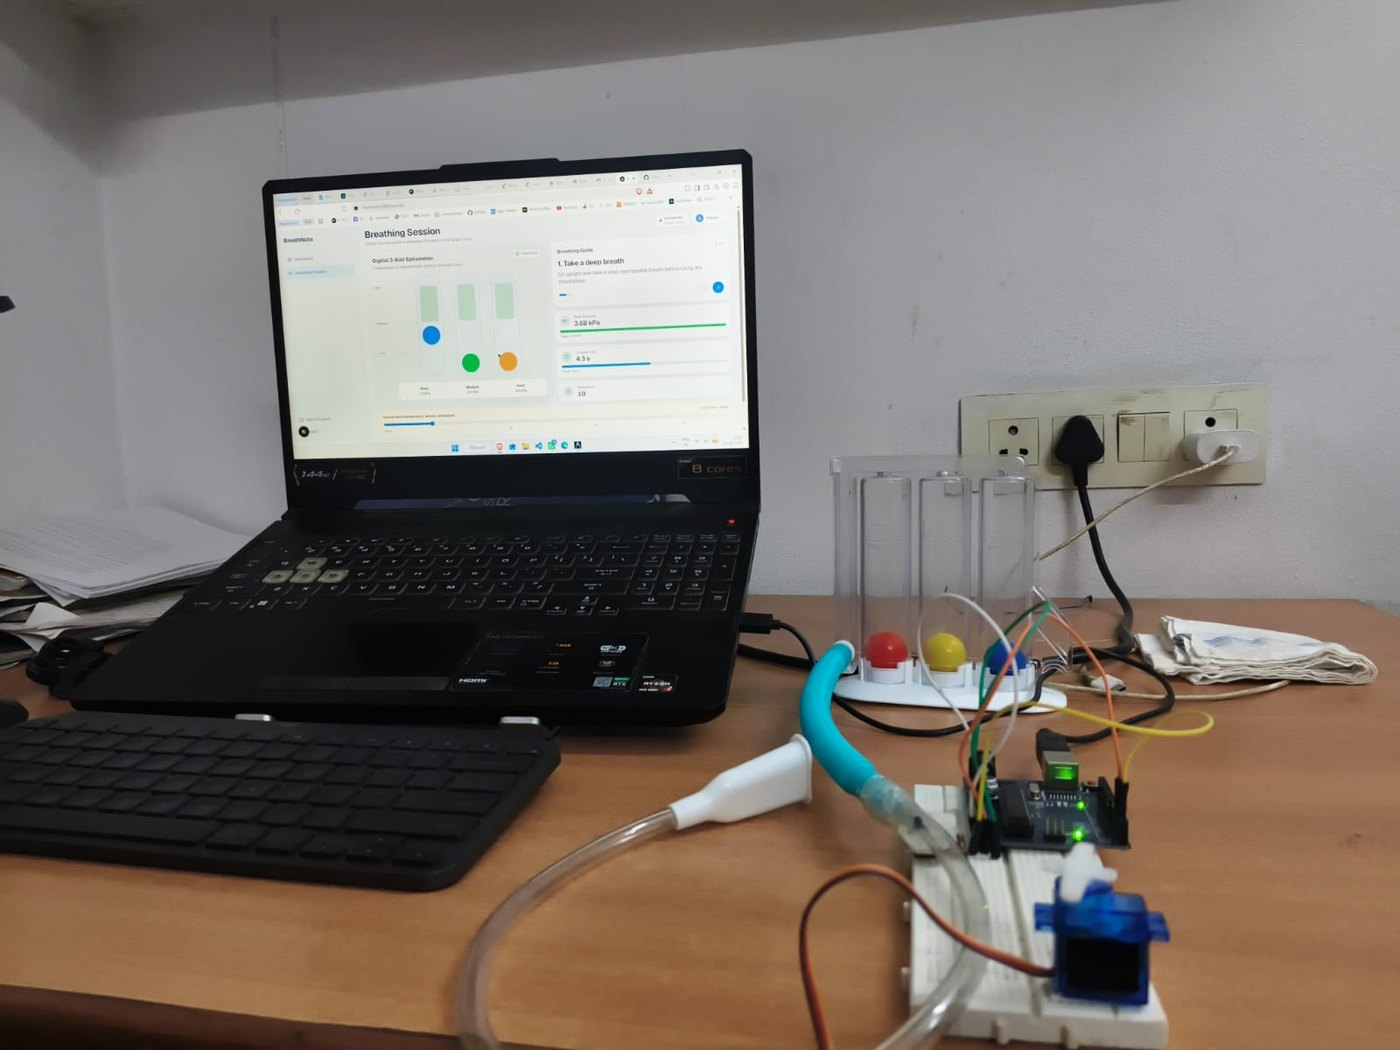
\includegraphics[width=0.48\linewidth]{figures/prototype.jpg}\hfill
  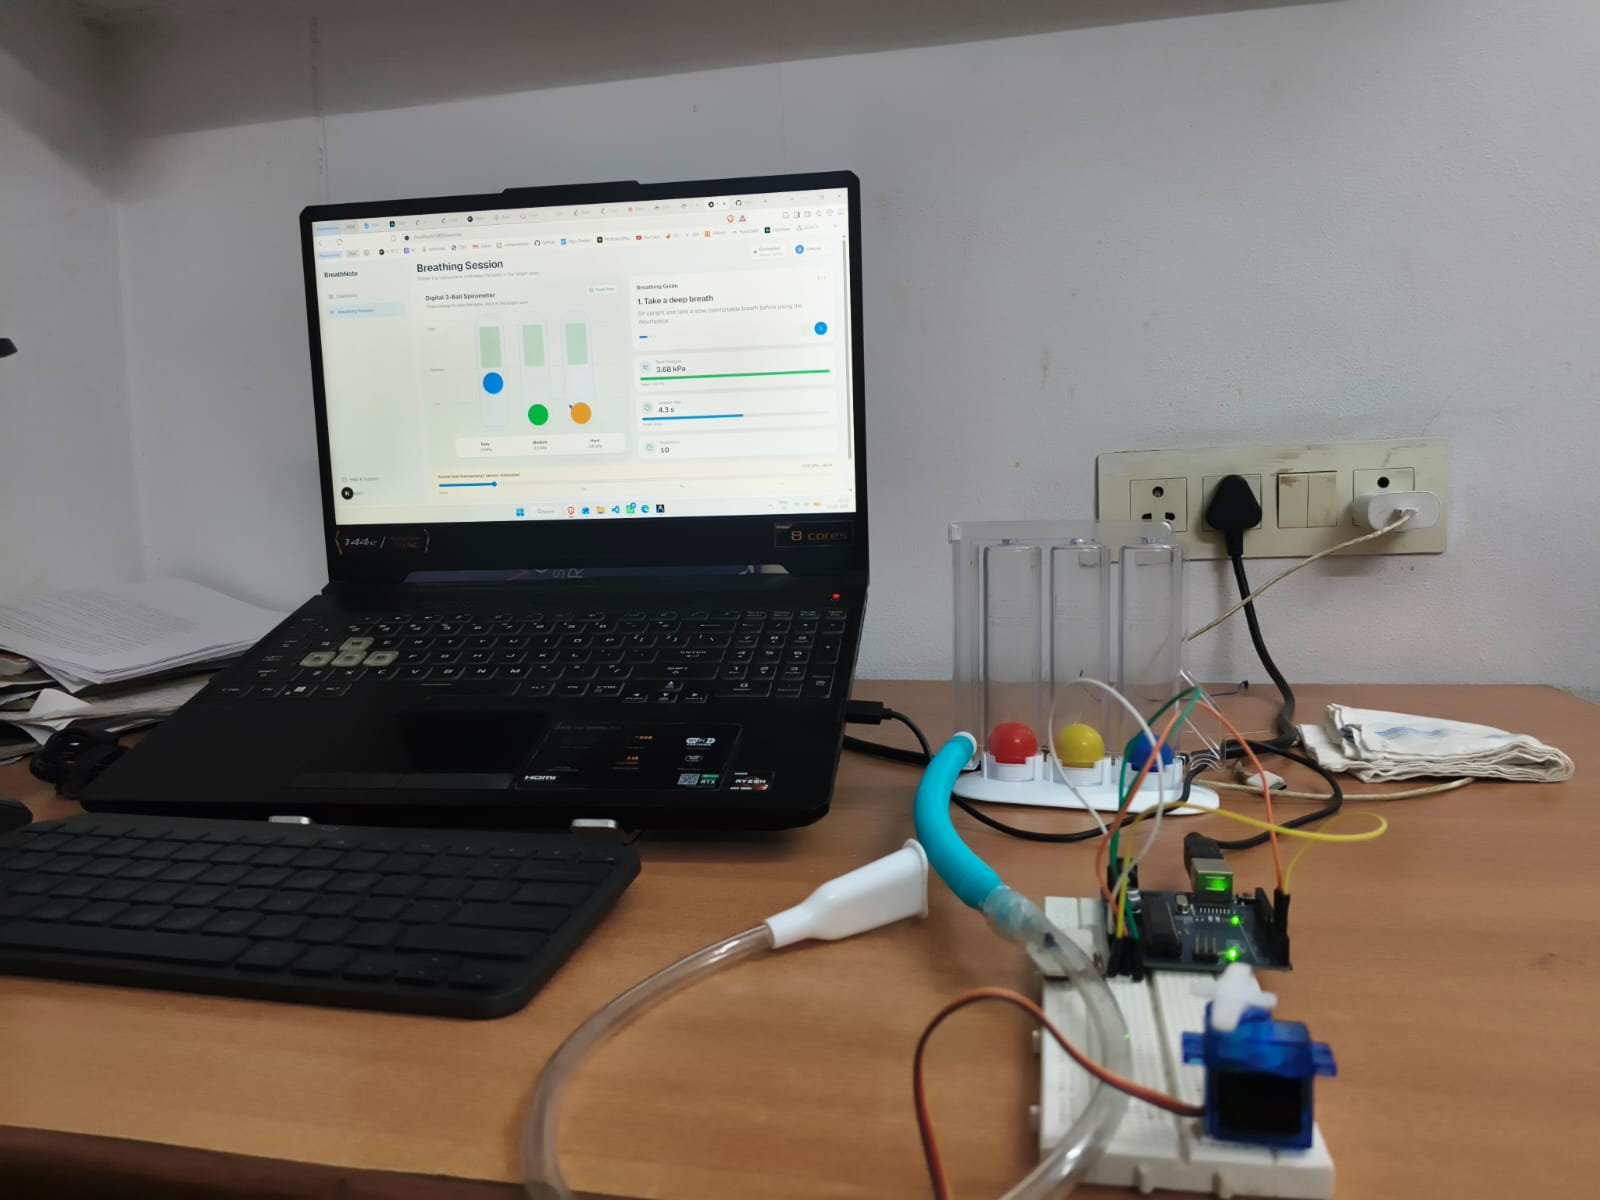
\includegraphics[width=0.48\linewidth]{figures/lab_setup.png}
  \caption{The working BreathNote prototype: a standard 3-ball incentive spirometer with the add-on, and the live breathing session on a laptop.}
  \label{fig:prototype}
\end{figure}

\subsection{How BreathNote addresses the challenges}
\begin{itemize}
  \item \textbf{Repetitive exercise:} every breath plays a musical glide and builds a chord, so each repetition feels different and rewarding.
  \item \textbf{Low motivation:} the music is a reward that grows with effort and hold time.
  \item \textbf{Visual-only feedback:} sound feedback works even with the eyes closed.
  \item \textbf{No data:} every session and every repetition is saved.
  \item \textbf{No progress view:} a personal dashboard with a progress chart and a consistency tracker.
  \item \textbf{No reminders:} email reminders at the times and days the patient chooses.
  \item \textbf{No report for the doctor:} a downloadable PDF progress report.
  \item \textbf{Lack of digital rehabilitation support:} a digital platform with a guided breathing session, live feedback, progress tracking, reminders and reports supports the patient's therapy, in hospital and at home.
\end{itemize}

% =====================================================================
\section{Innovation}
\label{sec:innovation}

\begin{enumerate}
  \item \textbf{The breath plays the music.} The music is not in the background. The breath controls the pitch, the clarity (noise to note) and the harmony. Research shows that music changes breathing only when it responds to the user \cite{bhandari}.
  \item \textbf{Harmony that builds with effort.} Each ball that reaches the top leaves its note sounding. The chord grows from one note to two to three. The patient \emph{hears} their progress during each breath. To our knowledge, breath-driven harmony of this kind has not been built into an incentive spirometer before.
  \item \textbf{Notes chosen from Indian music and acoustics.} Ga, Pa and \Sah{} are tuned in just intonation (5:4, 3:2, 2:1) from a reference Sa, the way a tanpura is tuned. They are the notes of the natural harmonic series of Sa, so they sound consonant and calming (Section~\ref{sec:music}).
  \item \textbf{It rewards good technique.} The music climbs only with stronger effort and keeps sounding only while the breath is held. This encourages the slow, sustained breath that doctors want.
  \item \textbf{It records and reports every breath.} Sessions and repetitions are saved; reminders and a PDF report connect the patient to the doctor.
  \item \textbf{Low-cost sensing found by testing.} We tested commercial sensors, a Venturi tube and turbine sensors, and chose a single pressure sensor in a closed tube that works at the low effort levels patients produce (Section~\ref{sec:sensor}).
\end{enumerate}

\begin{table}[H]
\centering
\caption{Conventional incentive spirometer compared with BreathNote.}
\label{tab:compare}
\footnotesize
\renewcommand{\arraystretch}{1.05}
\begin{tabularx}{\linewidth}{@{}P{2.4cm} P{4.6cm} L@{}}
\toprule
\textbf{Feature} & \textbf{Conventional 3-ball spirometer} & \textbf{BreathNote} \\
\midrule
Feedback       & Balls rise (visual only)     & Virtual balls and breath-driven music \\
Motivation     & Sight of the balls rising    & Musical glide and growing harmony as a reward \\
Data recorded  & Nothing                      & Every session and repetition: peak, level, hold time \\
Tracking       & Not possible                 & Dashboard with progress chart and history \\
Reminders      & None                         & Email reminders on chosen days and times \\
For the doctor & Only if they watch in person & Downloadable PDF progress report \\
Device         & Standard device              & Same device with a low-cost sensor add-on \\
\bottomrule
\end{tabularx}
\end{table}

% =====================================================================
\section{Features}
\label{sec:features}

\begin{itemize}
  \item \textbf{Breathing sessions:} guided sessions with a virtual 3-ball spirometer whose balls rise with the patient's breath, plus start, pause, restart and end controls.
  \item \textbf{Breath-driven music:} music that follows the breath and builds into a harmony as each level is reached, with a mute option.
  \item \textbf{Breathing guide:} step-by-step instructions shown on the session screen.
  \item \textbf{Live performance metrics:} peak pressure, longest hold, repetitions and session time, shown during the session against targets.
  \item \textbf{Automatic session recording:} every session and every breath is counted and saved.
  \item \textbf{Personalised dashboard:} summary cards, recent sessions, a progress chart, a 14-day consistency tracker and the full session history.
  \item \textbf{Reminders:} the patient sets exercise reminders for chosen times and days.
  \item \textbf{Notifications:} an email notification is sent when each exercise is due.
  \item \textbf{Progress reports:} a downloadable PDF report for the last week, month, six months or all time, to share with the doctor.
\end{itemize}

% =====================================================================
\section{Implementation}
\label{sec:impl}

\subsection{System Architecture}
\label{sec:arch}

BreathNote has three layers (Figure~\ref{fig:arch}):
\begin{enumerate}
  \item \textbf{Hardware layer:} the patient breathes into the mouthpiece; the HX710B sensor measures the air pressure in the tube; the Arduino Uno reads it and sends the raw values over USB serial.
  \item \textbf{Software and browser layer:} the Node.js bridge on the laptop calibrates the values and streams them over a WebSocket to the web application in the browser. The browser shows the virtual spirometer, plays the music and counts repetitions.
  \item \textbf{Backend and database layer:} the Next.js server checks logins, validates and saves sessions, sends reminder emails and builds PDF reports. Data is stored in PostgreSQL in the cloud.
\end{enumerate}

\begin{figure}[H]
  \centering
  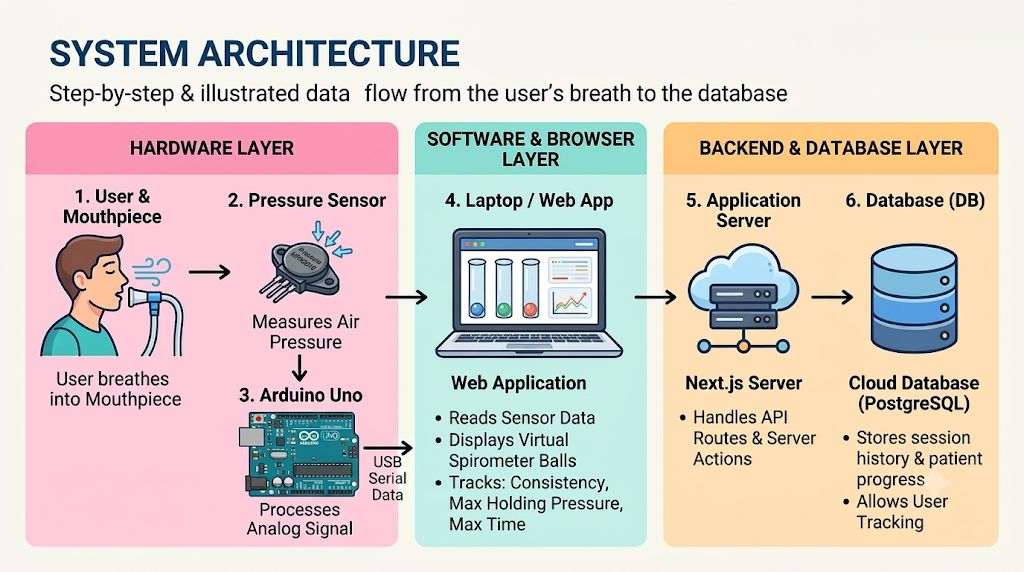
\includegraphics[width=0.95\linewidth]{figures/architecture.png}
  \caption{System architecture: hardware, software/browser, and backend/database layers.}
  \label{fig:arch}
\end{figure}

\begin{figure}[H]
\centering
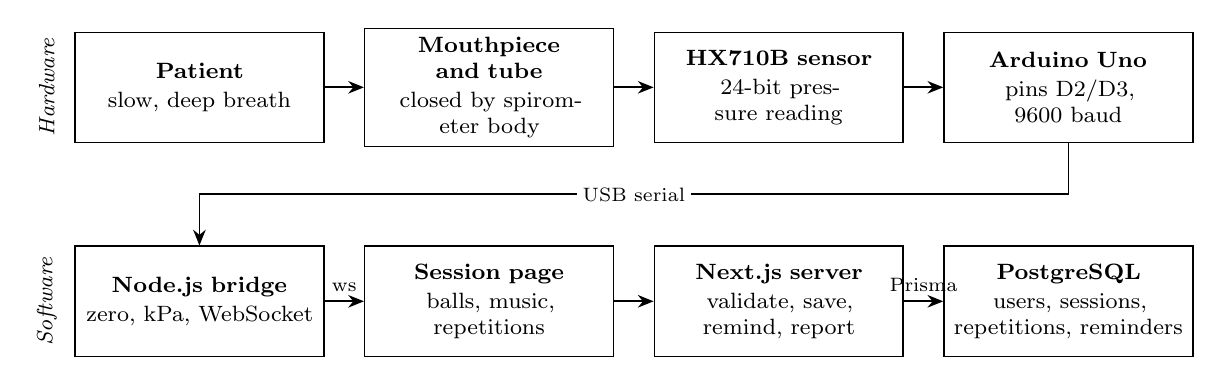
\begin{tikzpicture}[
    node distance=5mm,
    box/.style={draw=black, fill=white, line width=0.5pt, align=center,
                text width=2.95cm, minimum height=14mm, inner sep=3pt,
                font=\footnotesize},
    arr/.style={-{Stealth[length=2mm, width=1.6mm]}, line width=0.6pt},
    lane/.style={rotate=90, font=\footnotesize\itshape}
  ]
  \node[box]                (a1) {\textbf{Patient}\\[1pt] slow, deep breath};
  \node[box, right=of a1]   (a2) {\textbf{Mouthpiece and tube}\\[1pt] closed by spirometer body};
  \node[box, right=of a2]   (a3) {\textbf{HX710B sensor}\\[1pt] 24-bit pressure reading};
  \node[box, right=of a3]   (a4) {\textbf{Arduino Uno}\\[1pt] pins D2/D3, 9600 baud};
  \node[box, below=13mm of a1] (b1) {\textbf{Node.js bridge}\\[1pt] zero, kPa, WebSocket};
  \node[box, right=of b1]      (b2) {\textbf{Session page}\\[1pt] balls, music, repetitions};
  \node[box, right=of b2]      (b3) {\textbf{Next.js server}\\[1pt] validate, save, remind, report};
  \node[box, right=of b3]      (b4) {\textbf{PostgreSQL}\\[1pt] users, sessions, repetitions, reminders};
  \draw[arr] (a1) -- (a2);
  \draw[arr] (a2) -- (a3);
  \draw[arr] (a3) -- (a4);
  \draw[arr] (a4.south) -- ++(0,-6.5mm)
     -| node[pos=0.25, fill=white, inner sep=2pt, font=\scriptsize] {USB serial}
     (b1.north);
  \draw[arr] (b1) -- node[above, font=\scriptsize]{ws} (b2);
  \draw[arr] (b2) -- (b3);
  \draw[arr] (b3) -- node[above, font=\scriptsize]{Prisma} (b4);
  \node[lane] at ($(a1.west)+(-3.5mm,0)$) {Hardware};
  \node[lane] at ($(b1.west)+(-3.5mm,0)$) {Software};
\end{tikzpicture}
\caption{Data flow from the patient's breath to the database.}
\label{fig:flow}
\end{figure}

\subsubsection*{Software technologies used}

\begin{table}[H]
\centering
\caption{Software technologies used in BreathNote.}
\label{tab:tech}
\footnotesize
\renewcommand{\arraystretch}{1.05}
\begin{tabularx}{\linewidth}{@{}P{2.0cm} P{4.4cm} L@{}}
\toprule
\textbf{Layer} & \textbf{Technology} & \textbf{Used for} \\
\midrule
Bridge   & Node.js, TypeScript, serialport, ws & Reads USB serial data, converts it to kPa and streams it live to the browser \\
Frontend & Next.js, React, TypeScript, Tailwind CSS & Web application pages, logic and styling \\
         & Recharts                 & Progress chart on the dashboard \\
         & Web Audio API            & Breath-driven music, generated live in the browser \\
Backend  & Next.js Server Actions   & Saving sessions, reminders and login \\
         & Nodemailer + Gmail SMTP  & Reminder emails \\
         & React-PDF                & Downloadable progress report \\
Database & PostgreSQL (cloud), Prisma ORM & Stores users, sessions, repetitions and reminders \\
Security & bcrypt, JWT (HTTP-only cookie) & Password hashing and secure login \\
Design   & Figma                    & UI/UX design of all screens \\
\bottomrule
\end{tabularx}
\end{table}

\subsubsection*{Component list}
\label{sec:components}

\begin{table}[H]
\centering
\caption{Hardware components and why each is used.}
\label{tab:components}
\footnotesize
\renewcommand{\arraystretch}{1.05}
\begin{tabularx}{\linewidth}{@{}P{4.0cm} L@{}}
\toprule
\textbf{Component} & \textbf{Why we use it} \\
\midrule
3-ball incentive spirometer & The device patients already use; its body acts as the closed air container \\
HX710B pressure sensor module & Measures breathing pressure in the tube (24-bit, 0--40\,kPa); cheap and available in the ECE store \\
Arduino Uno & Reads the sensor and sends data to the laptop over USB; powers the sensor \\
Silicone tube and mouthpiece & Hygienic breathing interface; the tube seals around the sensor nozzle \\
Breadboard and jumper wires & Quick, solder-free wiring of the prototype \\
USB cable & Data link and 5\,V power from the laptop \\
Sealant / hot glue & Keeps the sensor joint airtight \\
Laptop (Chrome browser) & Runs the bridge, the web application and plays the music \\
\bottomrule
\end{tabularx}
\end{table}



\subsection{Figma UI/UX Design}
\label{sec:figma}

Before coding, we designed every screen in Figma (\href{\figmaurl}{link}). Our design goals were: \emph{calm} (soft blues and greens, lots of white space), \emph{simple} (large text, few buttons, one clear action per screen), and \emph{familiar} (the virtual spirometer looks like the real 3-ball device, with the same three ball colours).

\begin{figure}[H]
  \centering
  \begin{subfigure}[b]{0.49\linewidth}
    \centering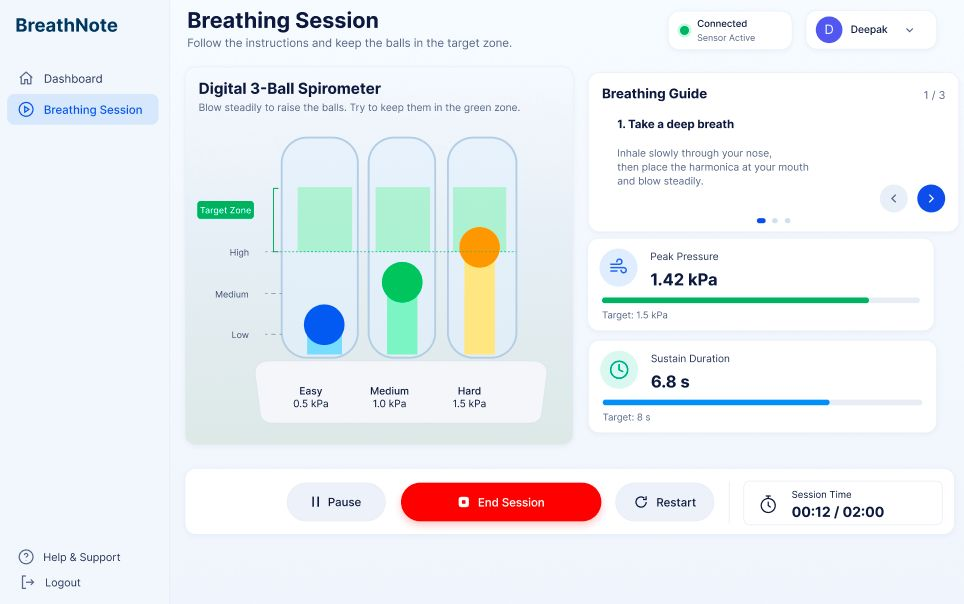
\includegraphics[width=\linewidth]{figures/figma_session.png}
    \caption{Breathing session screen.}
  \end{subfigure}\hfill
  \begin{subfigure}[b]{0.49\linewidth}
    \centering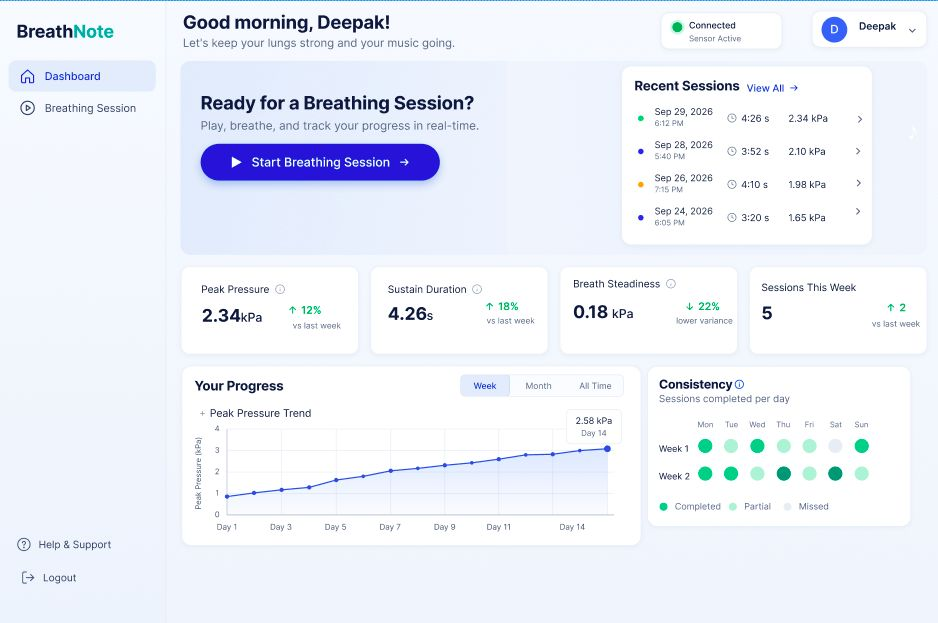
\includegraphics[width=\linewidth]{figures/figma_dashboard.png}
    \caption{Personal dashboard.}
  \end{subfigure}
  \caption{Figma designs of the two main screens.}
  \label{fig:figma}
\end{figure}

\begin{itemize}
  \item \textbf{Login / Sign-up screen} (Figure~\ref{fig:login}): a single card with the BreathNote name and tagline ``Breathe Better. Live Better.'' Tabs switch between login and sign-up.
  \item \textbf{Breathing session screen:} on the left, the digital 3-ball spirometer with a green \emph{target zone} and the Easy / Medium / Hard thresholds in kPa. On the right, the breathing guide and metric cards (peak pressure, longest hold, repetitions) with progress bars towards the targets. At the bottom, the control bar: Start/Pause, End Session, Restart, Sound on/off and the session timer. The top bar shows the sensor status.
  \item \textbf{Dashboard:} a greeting, a ``Ready for a breathing session?'' card with a large start button, recent sessions, four summary cards, the progress chart, the consistency tracker, reminders, report download and the full session history.
\end{itemize}

\begin{figure}[H]
  \centering
  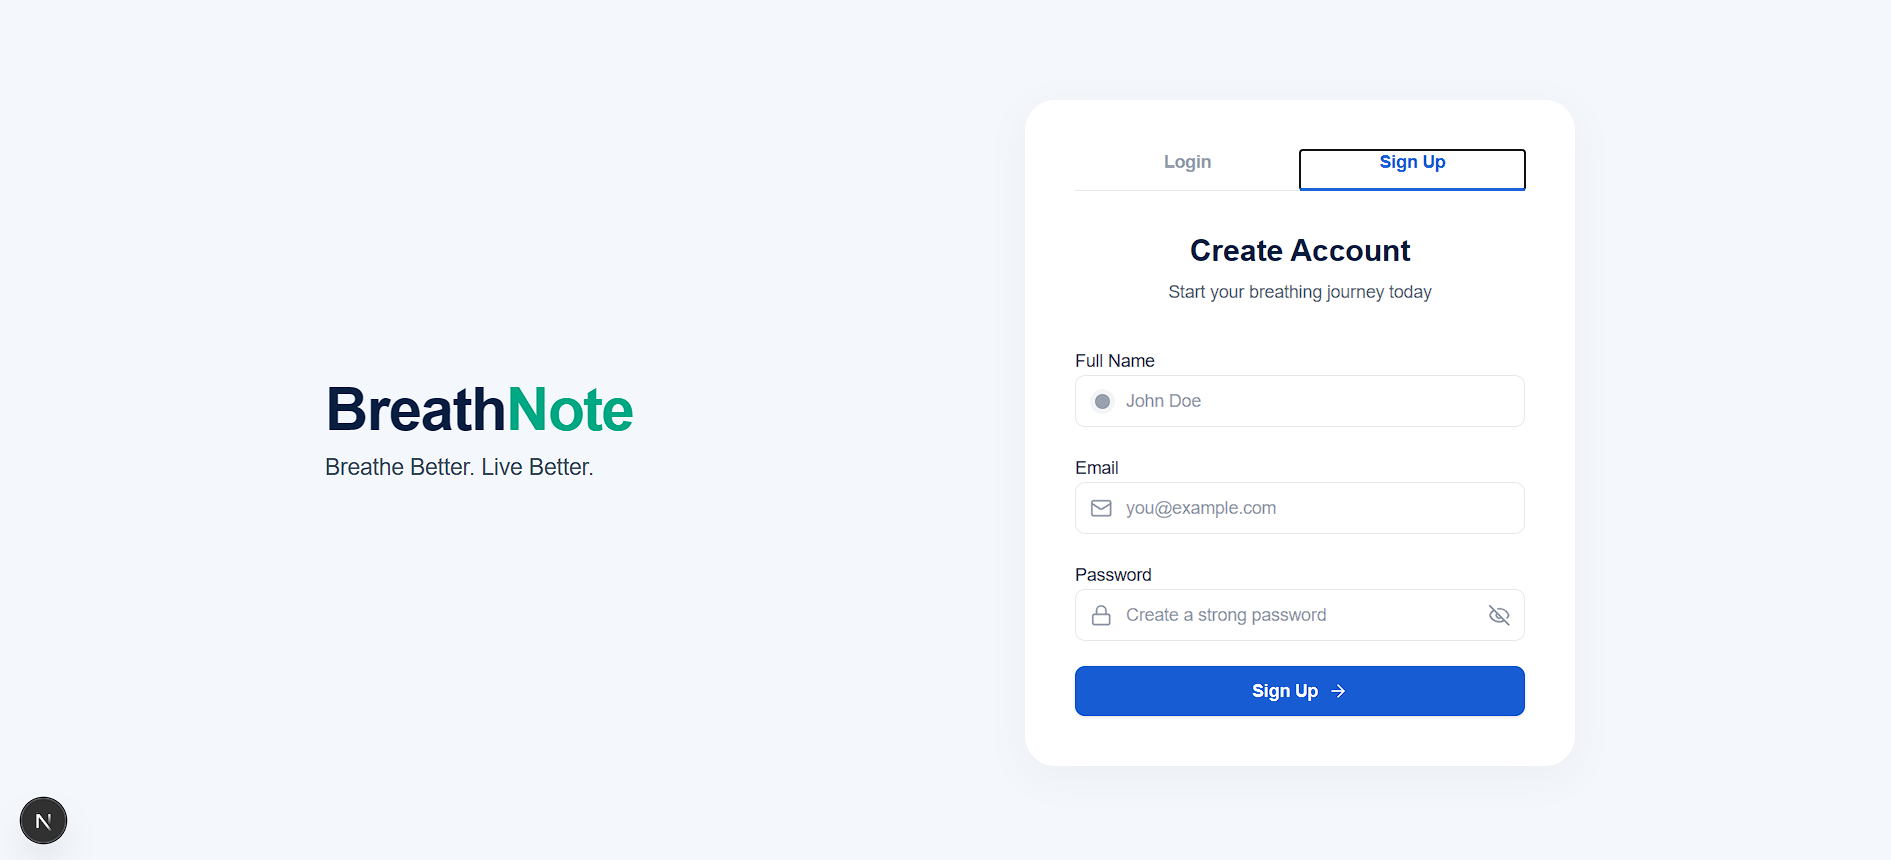
\includegraphics[width=0.62\linewidth]{figures/figma_login.png}
  \caption{Figma design of the login and sign-up screen.}
  \label{fig:login}
\end{figure}

\begin{figure}[H]
  \centering
  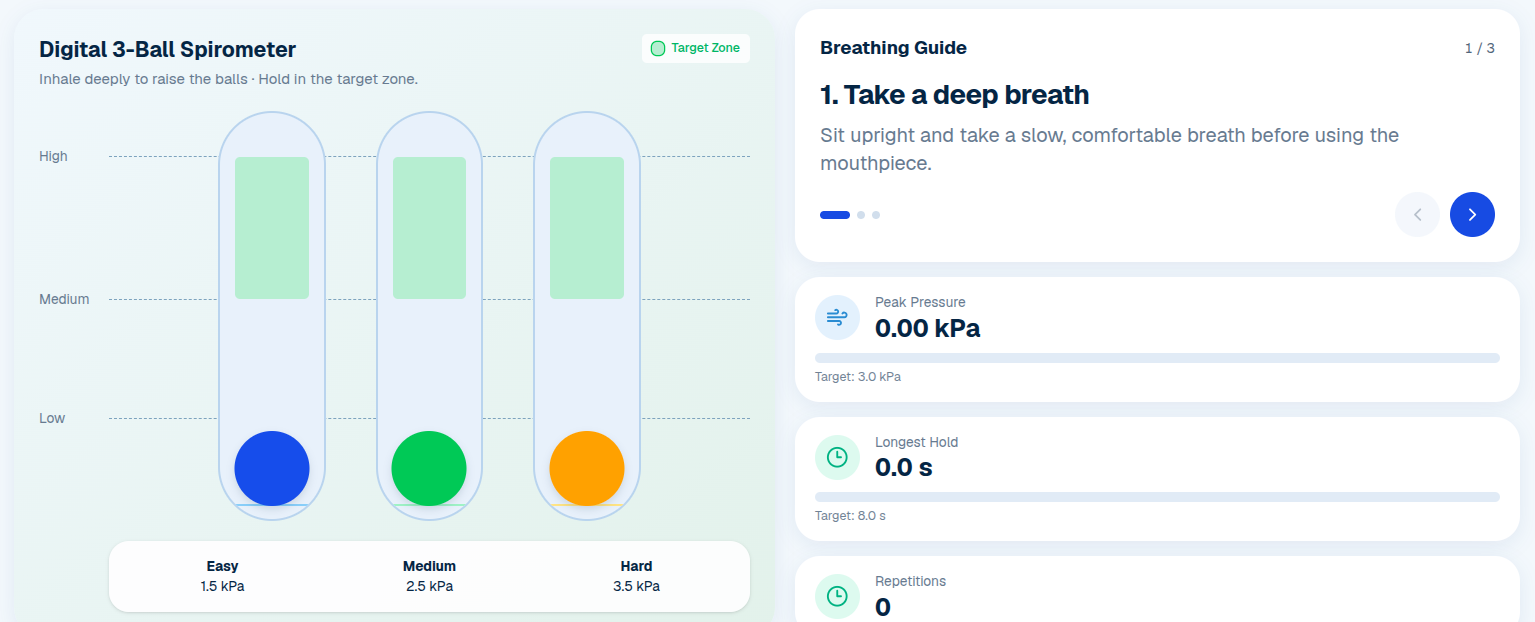
\includegraphics[width=0.49\linewidth]{figures/session.png}\hfill
  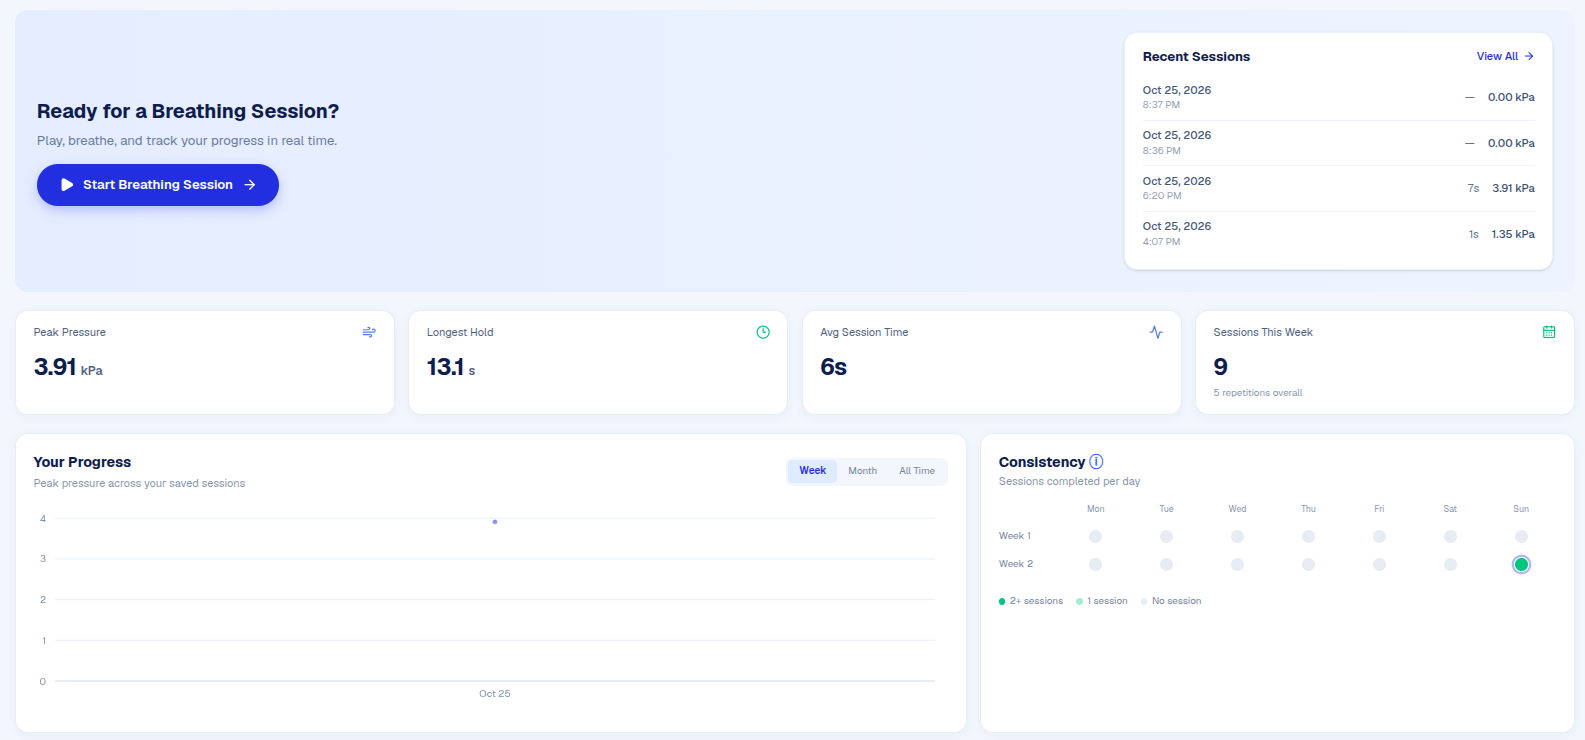
\includegraphics[width=0.49\linewidth]{figures/dashboard.png}
  \caption{The final built application. Left: the breathing session with live sensor data. Right: the personal dashboard.}
  \label{fig:screens}
\end{figure}

\subsection{Database Schema}
\label{sec:db}

BreathNote stores its data in a \textbf{PostgreSQL} database in the cloud. The database has four tables: one for users, one for sessions, one for the breaths inside each session, and one for reminders.

\textbf{1. \texttt{users} --- who the patient is.} Each patient needs their own account, so their data stays separate and private. This table stores the login details and the name shown on the dashboard.

\begin{table}[H]
\centering
\caption{Table \texttt{users}.}
\small
\begin{tabularx}{\linewidth}{@{}P{4.4cm} L@{}}
\toprule
\textbf{Column} & \textbf{What it stores} \\
\midrule
id & A unique ID for each user \\
name & The patient's name \\
email & Login email (also used for reminders) \\
password\_hash & The password in a secure, hidden form \\
created\_at, updated\_at & When the account was created and last changed \\
\bottomrule
\end{tabularx}
\end{table}

\textbf{2. \texttt{exercise\_sessions} --- one row for each practice session.} A session runs from \emph{Start Session} to \emph{End Session}. Saving a summary of each session lets the dashboard and reports show progress quickly.

\begin{table}[H]
\centering
\caption{Table \texttt{exercise\_sessions}.}
\small
\begin{tabularx}{\linewidth}{@{}P{4.4cm} L@{}}
\toprule
\textbf{Column} & \textbf{What it stores} \\
\midrule
id & A unique ID for each session \\
user\_id & Which user the session belongs to \\
start\_time, end\_time & When the session started and ended \\
duration\_seconds & How long the session was (without pauses) \\
max\_pressure\_achieved & The highest breathing pressure in the session (kPa) \\
max\_level\_reached & The highest level reached (Easy, Medium or Hard) \\
max\_level\_hold\_duration & The longest time a level was held \\
number\_of\_repetitions & How many breaths were taken \\
created\_at & When the session was saved \\
\bottomrule
\end{tabularx}
\end{table}

\textbf{3. \texttt{repetitions} --- one row for each breath.} The session table keeps only the best values. This table keeps the details of every single breath, so we can see how each breath went.

\begin{table}[H]
\centering
\caption{Table \texttt{repetitions}.}
\small
\begin{tabularx}{\linewidth}{@{}P{4.4cm} L@{}}
\toprule
\textbf{Column} & \textbf{What it stores} \\
\midrule
id & A unique ID for each breath \\
session\_id & Which session the breath belongs to \\
timestamp & When the breath started \\
max\_pressure & How strong the breath was (kPa) \\
level\_reached & The highest level reached in this breath \\
hold\_duration & How long the breath was held \\
\bottomrule
\end{tabularx}
\end{table}

\textbf{4. \texttt{reminders} --- the patient's exercise reminders.} Patients often forget their exercises, so they can set reminders. Each reminder stores its time and days, and remembers when it was last sent so it is sent only once a day.

\begin{table}[H]
\centering
\caption{Table \texttt{reminders}.}
\small
\begin{tabularx}{\linewidth}{@{}P{4.4cm} L@{}}
\toprule
\textbf{Column} & \textbf{What it stores} \\
\midrule
id & A unique ID for each reminder \\
user\_id & Which user set the reminder \\
hour, minute & The time of the reminder \\
days & The days of the week it is sent \\
timezone & The patient's timezone, so it arrives at the right local time \\
enabled & Whether the reminder is on or off \\
last\_sent\_on & The date it was last sent \\
created\_at & When the reminder was created \\
\bottomrule
\end{tabularx}
\end{table}

\subsection{Entity Relationships}
\label{sec:er}

The data follows a strict hierarchy (Figure~\ref{fig:er}):
\begin{itemize}
  \item \textbf{One user has many sessions} (1: N). Every session belongs to exactly one user.
  \item \textbf{One session has many repetitions} (1: N). Every repetition belongs to exactly one session.
  \item \textbf{One user has many reminders} (1: N).
\end{itemize}
This separates \emph{who} the user is from \emph{what} they did. The dashboard can show a summary (session rows) quickly, and the details (repetition rows) are kept for deeper analysis and future doctor views.

\begin{figure}[tbp]
\centering
\resizebox{0.78\linewidth}{!}{%
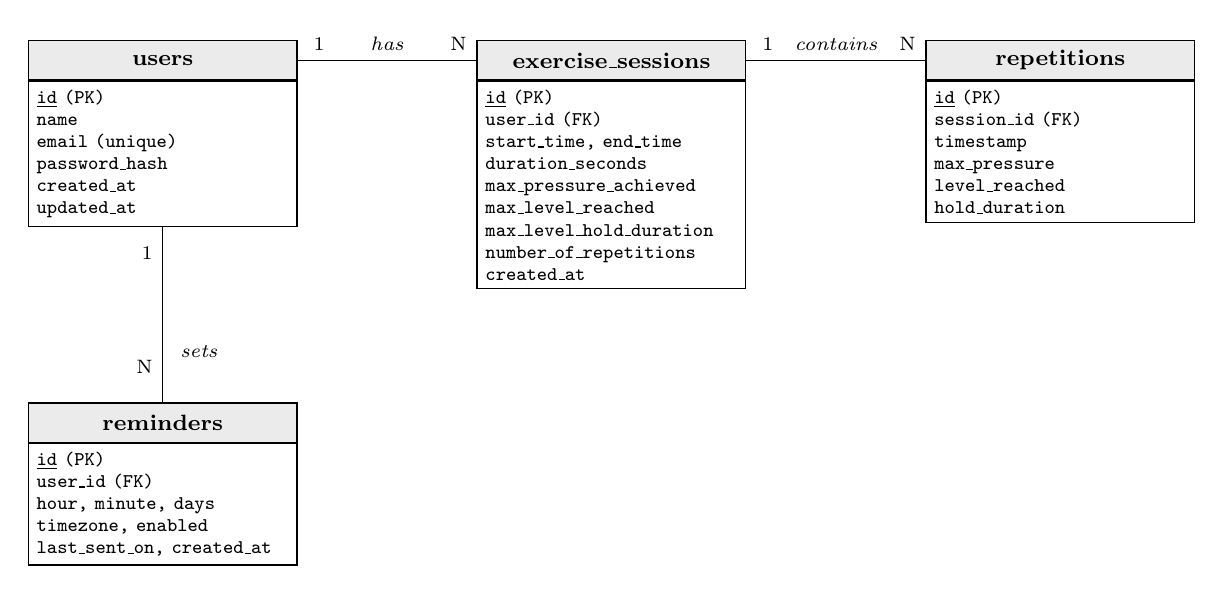
\begin{tikzpicture}[
   ent/.style={draw=black, line width=0.5pt, align=left, font=\scriptsize\ttfamily,
               inner sep=3pt, text width=3.2cm},
   hdr/.style={draw=black, fill=black!8, line width=0.5pt, font=\footnotesize\bfseries,
               minimum height=5mm, text width=3.2cm, align=center, inner sep=3pt},
   rel/.style={line width=0.6pt}]
  \node[hdr] (uh) at (0,0) {users};
  \node[ent, below=0pt of uh] (ub) {\underline{id} (PK)\\ name\\ email (unique)\\ password\_hash\\ created\_at\\ updated\_at};
  \node[hdr] (sh) at (5.7,0) {exercise\_sessions};
  \node[ent, below=0pt of sh] (sb) {\underline{id} (PK)\\ user\_id (FK)\\ start\_time, end\_time\\ duration\_seconds\\ max\_pressure\_achieved\\ max\_level\_reached\\ max\_level\_hold\_duration\\ number\_of\_repetitions\\ created\_at};
  \node[hdr] (rh) at (11.4,0) {repetitions};
  \node[ent, below=0pt of rh] (rb) {\underline{id} (PK)\\ session\_id (FK)\\ timestamp\\ max\_pressure\\ level\_reached\\ hold\_duration};
  \node[hdr] (mh) at (0,-4.6) {reminders};
  \node[ent, below=0pt of mh] (mb) {\underline{id} (PK)\\ user\_id (FK)\\ hour, minute, days\\ timezone, enabled\\ last\_sent\_on, created\_at};
  \draw[rel] (uh.east) -- node[above, font=\scriptsize, pos=0.12]{1} node[above, font=\scriptsize\itshape, pos=0.5]{has} node[above, font=\scriptsize, pos=0.9]{N} (sh.west);
  \draw[rel] (sh.east) -- node[above, font=\scriptsize, pos=0.12]{1} node[above, font=\scriptsize\itshape, pos=0.5]{contains} node[above, font=\scriptsize, pos=0.9]{N} (rh.west);
  \draw[rel] (ub.south) -- node[left, font=\scriptsize, pos=0.15]{1} node[left, font=\scriptsize, pos=0.8]{N} (mh.north);
      \node[font=\scriptsize\itshape, right] at (0.1,-3.7) {sets};
\end{tikzpicture}%
}
\caption{Entity--relationship diagram. PK = primary key, FK = foreign key.}
\label{fig:er}
\end{figure}

\subsection{Working of the System: From Mouthpiece to Database}
\label{sec:working}

This is the path of one breath, step by step.

\begin{enumerate}
  \item \textbf{Breathe.} The patient breathes slowly and deeply through the mouthpiece.
  \item \textbf{Pressure changes.} The far end of the tube is closed by the spirometer body, so the breath changes the pressure along the whole tube.
  \item \textbf{Sense.} The HX710B sensor, sealed into the tube, measures this pressure as a number (raw count).
  \item \textbf{Read.} The Arduino reads the sensor and sends each value to the laptop over USB.
  \item \textbf{Calibrate.} The bridge learns the zero level in the first 3 seconds, then converts each reading to kPa and sends it live to the browser:
  \[
    p\,[\text{kPa}] = \frac{\text{raw} - \text{zero}}{\text{counts per kPa}}.
  \]
  \item \textbf{Move the balls.} The three balls rise and fall with the pressure (Section~\ref{sec:feat-visual}).
  \item \textbf{Play the music.} The music follows the balls and builds into a harmony (Section~\ref{sec:music-impl}).
  \item \textbf{Count repetitions.} Each breath above 0.5\,kPa is one repetition; its peak pressure, highest level and hold time are recorded.
  \item \textbf{End and save.} On \emph{End Session}, the session and its repetitions are sent to the server.
  \item \textbf{Store.} The session and all its repetitions are saved in the database.
  \item \textbf{Show.} The dashboard updates with the new session.
\end{enumerate}

\subsection{End-to-End Flow: Sequence Diagram}
\label{sec:seq}

Figure~\ref{fig:seq} shows the same flow as a sequence diagram: who sends what to whom, in time order from top to bottom.

\begin{figure}[H]
\centering
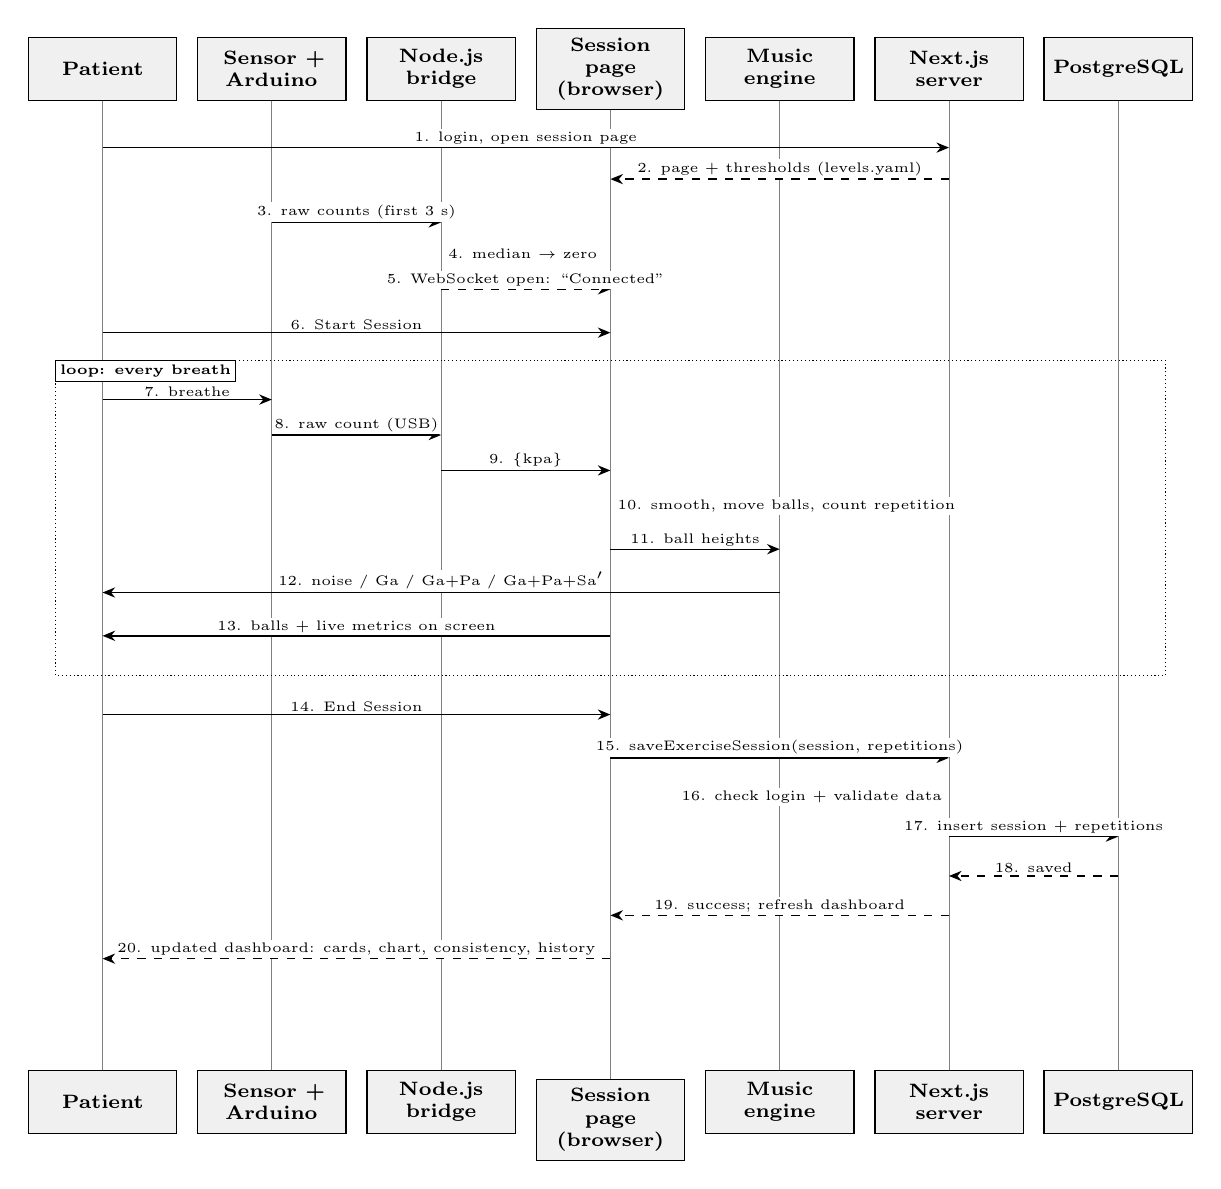
\begin{tikzpicture}[
    actor/.style={draw=black, fill=black!6, line width=0.5pt, font=\scriptsize\bfseries,
                  align=center, minimum width=1.75cm, minimum height=8mm, text width=1.65cm},
    msg/.style={-{Stealth[length=1.6mm, width=1.3mm]}, line width=0.5pt},
    ret/.style={-{Stealth[length=1.6mm, width=1.3mm]}, line width=0.5pt, dashed},
    lbl/.style={font=\tiny, fill=white, inner sep=1pt}]
  % Actors
  \foreach \x/\n/\t in {0/P/Patient, 2.15/S/{Sensor +\\Arduino}, 4.3/B/{Node.js\\bridge}, 6.45/W/{Session page\\(browser)}, 8.6/A/{Music\\engine}, 10.75/N/{Next.js\\server}, 12.9/D/{PostgreSQL}}{
    \node[actor] (\n) at (\x,0) {\t};
    \draw[line width=0.3pt, black!50] (\n.south) -- ++(0,-12.3);
    \node[actor, anchor=north] at ($(\n.south)+(0,-12.3)$) {\t};
  }
  % Messages (y positions)
  \draw[msg] (0,-1.0) -- node[lbl, above]{1. login, open session page} (10.75,-1.0);
  \draw[ret] (10.75,-1.4) -- node[lbl, above]{2. page + thresholds (levels.yaml)} (6.45,-1.4);
  \draw[msg] (2.15,-1.95) -- node[lbl, above]{3. raw counts (first 3 s)} (4.3,-1.95);
  \node[lbl, right] at (4.35,-2.35) {4. median $\rightarrow$ zero};
  \draw[ret] (4.3,-2.8) -- node[lbl, above]{5. WebSocket open: ``Connected''} (6.45,-2.8);
  \draw[msg] (0,-3.35) -- node[lbl, above]{6. Start Session} (6.45,-3.35);
  % loop box
  \draw[line width=0.4pt, densely dotted] (-0.6,-3.7) rectangle (13.5,-7.7);
  \node[font=\tiny\bfseries, anchor=north west, draw, fill=white, inner sep=1.5pt] at (-0.6,-3.7) {loop: every breath};
  \draw[msg] (0,-4.2) -- node[lbl, above]{7. breathe} (2.15,-4.2);
  \draw[msg] (2.15,-4.65) -- node[lbl, above]{8. raw count (USB)} (4.3,-4.65);
  \draw[msg] (4.3,-5.1) -- node[lbl, above]{9. \{kpa\}} (6.45,-5.1);
  \node[lbl, right] at (6.5,-5.55) {10. smooth, move balls, count repetition};
  \draw[msg] (6.45,-6.1) -- node[lbl, above]{11. ball heights} (8.6,-6.1);
  \draw[msg] (8.6,-6.65) -- node[lbl, above]{12. noise / Ga / Ga+Pa / Ga+Pa+\Sah} (0,-6.65);
  \draw[msg] (6.45,-7.2) -- node[lbl, above]{13. balls + live metrics on screen} (0,-7.2);
  % End
  \draw[msg] (0,-8.2) -- node[lbl, above]{14. End Session} (6.45,-8.2);
  \draw[msg] (6.45,-8.75) -- node[lbl, above]{15. saveExerciseSession(session, repetitions)} (10.75,-8.75);
  \node[lbl, left] at (10.7,-9.25) {16. check login + validate data};
  \draw[msg] (10.75,-9.75) -- node[lbl, above]{17. insert session + repetitions} (12.9,-9.75);
  \draw[ret] (12.9,-10.25) -- node[lbl, above]{18. saved} (10.75,-10.25);
  \draw[ret] (10.75,-10.75) -- node[lbl, above]{19. success; refresh dashboard} (6.45,-10.75);
  \draw[ret] (6.45,-11.3) -- node[lbl, above]{20. updated dashboard: cards, chart, consistency, history} (0,-11.3);
\end{tikzpicture}
\caption{End-to-end sequence of one breathing session.}
\label{fig:seq}
\end{figure}

\begin{figure}[H]
\centering
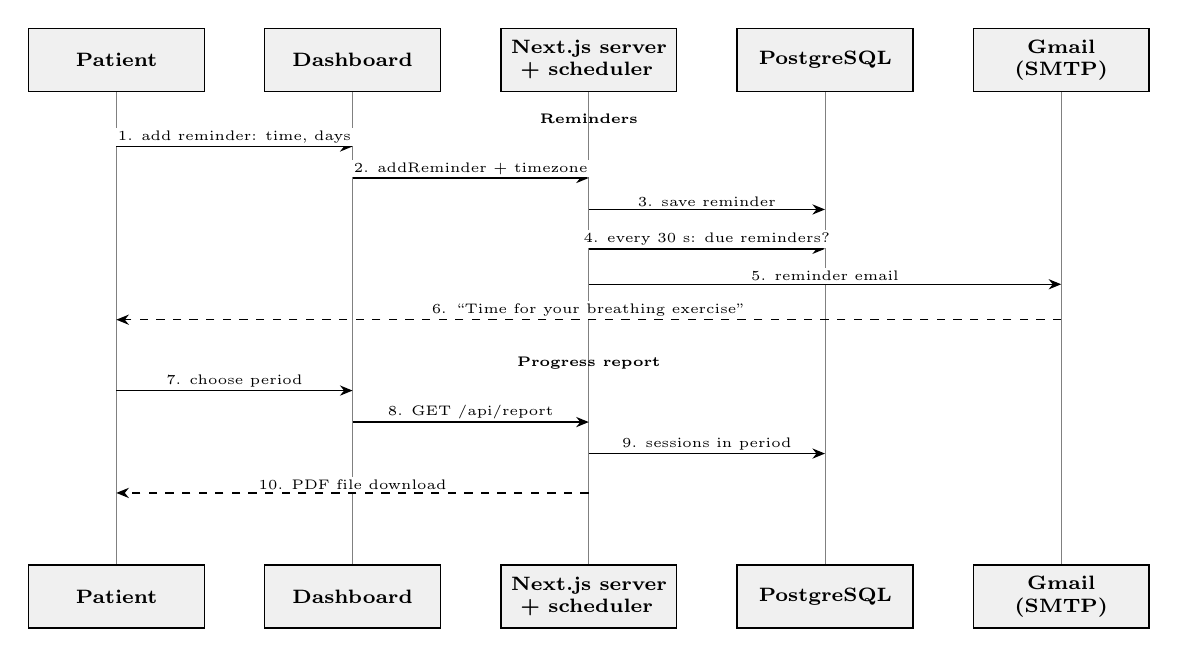
\begin{tikzpicture}[
    actor/.style={draw=black, fill=black!6, line width=0.5pt, font=\scriptsize\bfseries,
                  align=center, minimum width=2.1cm, minimum height=8mm, text width=2.0cm},
    msg/.style={-{Stealth[length=1.6mm, width=1.3mm]}, line width=0.5pt},
    ret/.style={-{Stealth[length=1.6mm, width=1.3mm]}, line width=0.5pt, dashed},
    lbl/.style={font=\tiny, fill=white, inner sep=1pt}]
  \foreach \x/\n/\t in {0/P/Patient, 3/W/Dashboard, 6/N/{Next.js server\\+ scheduler}, 9/D/PostgreSQL, 12/G/{Gmail\\(SMTP)}}{
    \node[actor] (\n) at (\x,0) {\t};
    \draw[line width=0.3pt, black!50] (\n.south) -- ++(0,-6.0);
    \node[actor, anchor=north] at ($(\n.south)+(0,-6.0)$) {\t};
  }
  \node[font=\tiny\bfseries] at (6,-0.75) {Reminders};
  \draw[msg] (0,-1.1) -- node[lbl, above]{1. add reminder: time, days} (3,-1.1);
  \draw[msg] (3,-1.5) -- node[lbl, above]{2. addReminder + timezone} (6,-1.5);
  \draw[msg] (6,-1.9) -- node[lbl, above]{3. save reminder} (9,-1.9);
  \draw[msg] (6,-2.4) -- node[lbl, above]{4. every 30 s: due reminders?} (9,-2.4);
  \draw[msg] (6,-2.85) -- node[lbl, above]{5. reminder email} (12,-2.85);
  \draw[ret] (12,-3.3) -- node[lbl, above]{6. ``Time for your breathing exercise''} (0,-3.3);
  \node[font=\tiny\bfseries] at (6,-3.85) {Progress report};
  \draw[msg] (0,-4.2) -- node[lbl, above]{7. choose period} (3,-4.2);
  \draw[msg] (3,-4.6) -- node[lbl, above]{8. GET /api/report} (6,-4.6);
  \draw[msg] (6,-5.0) -- node[lbl, above]{9. sessions in period} (9,-5.0);
  \draw[ret] (6,-5.5) -- node[lbl, above]{10. PDF file download} (0,-5.5);
\end{tikzpicture}
\caption{Sequence for reminders and the progress report.}
\label{fig:seq2}
\end{figure}

\subsection{Implementation of Each Feature}
\label{sec:features-impl}

BreathNote is made of several features that work together. Some of them work in the background, such as reading and calibrating the sensor, and some are seen directly by the patient, such as the breathing screen, the music and the dashboard. Together they cover the patient's full journey:

\begin{enumerate}
  \item \textbf{Before the exercise:} the patient logs in to their own account and gets a reminder when it is time to exercise.
  \item \textbf{During the exercise:} the sensor measures every breath, the virtual balls rise on the screen, the music builds into a harmony, and the live metrics show how well the patient is doing.
  \item \textbf{After the exercise:} the session is checked and saved, the dashboard shows the patient's progress, and a progress report can be downloaded for the doctor.
\end{enumerate}

We built each feature to solve one of the problems described in Section~\ref{sec:problem}: boring exercise, no motivation, no record of performance, and no information for the doctor. We also kept three goals in mind for every feature:
\begin{itemize}
  \item \textbf{Simple to use:} the patient should not need any training; the screens look like the real device and need only a few clicks.
  \item \textbf{Reliable:} only real breathing data is used, and wrong or impossible values are never saved.
  \item \textbf{Private:} each patient sees only their own data.
\end{itemize}

\subsubsection{Breathing session and repetitions}
\label{sec:feat-visual}
A \textbf{breathing session} is one complete practice, from clicking \emph{Start Session} to clicking \emph{End Session}. Inside one session, the patient takes many deep breaths; each deep breath is called a \textbf{repetition}.

\textbf{How we built it.}
\begin{itemize}
  \item The session screen shows a \textbf{virtual 3-ball spirometer}. The three balls (blue, green and orange) stand for three levels: \textbf{Easy, Medium and Hard}. They rise one after another as the breath gets stronger, just like the real device. The level targets (1.5, 2.5 and 3.5\,kPa) are kept in one settings file, so they can be changed for each patient.
  \item The patient can \textbf{start, pause, restart and end} the session. The session timer counts only active time, not pauses.
  \item A \textbf{repetition starts} when the breath becomes stronger than 0.5\,kPa and \textbf{ends} when the patient relaxes and it falls back below 0.5\,kPa. This small threshold ignores normal breathing and noise, so only real exercise breaths are counted.
  \item For \textbf{each repetition}, the app records: the \emph{peak pressure} (how strong the breath was), the \emph{highest level} reached (Easy, Medium or Hard), and the \emph{longest hold} (how long the patient stayed at one level).
  \item During the session, live cards show the \textbf{peak pressure} (target 3.0\,kPa), the \textbf{longest hold} (target 8\,s), the \textbf{number of repetitions} and the \textbf{session time}.
  \item When the patient clicks \emph{End Session}, the session and all its repetitions are saved. The server also calculates a \textbf{session summary}: the best peak, the highest level, the longest hold and the total number of repetitions.
\end{itemize}

\textbf{Use:} The patient sees a familiar picture and an immediate target on every breath. Recording each repetition separately shows not only how much the patient practised, but also how good each breath was.

\subsubsection{Breathing guide}
A card on the session screen that teaches the correct technique, one step at a time. The patient can move forward and back through six steps:
\begin{enumerate}
  \item \textbf{Get ready:} sit upright on the edge of the bed or a chair, hold the spirometer upright and breathe out normally.
  \item \textbf{Seal the mouthpiece:} place the mouthpiece in the mouth and close the lips tightly around it.
  \item \textbf{Breathe in slowly and deeply:} so that the balls rise towards the top; if they shoot up too fast, slow down.
  \item \textbf{Hold, then relax:} hold the breath for 3--5 seconds, then remove the mouthpiece and breathe out normally.
  \item \textbf{Rest and repeat:} rest with a few normal breaths and repeat 10 or more times; after each set of 10, cough a few times to clear the lungs.
  \item \textbf{Make it a habit:} do a set every 1--2 hours while awake; stop and rest if light-headed, and tell the doctor if the target is often missed.
\end{enumerate}

\textbf{Use:} The patient learns the right technique without needing a nurse beside them, which is especially useful at home.

\subsubsection{Integration of music}
During the session, the patient's breath plays music. The sound follows the three balls:
\begin{itemize}
  \item \textbf{Sa is not played}: it is only the reference pitch from which Ga, Pa and the upper Sa are calculated;
  \item weak effort sounds like soft \textbf{breath noise}, which turns into a clear \textbf{Ga} as the blue ball rises;
  \item the green ball makes the pitch glide up to \textbf{Pa}, while Ga keeps sounding (\textbf{Ga\,+\,Pa});
  \item the orange ball makes the pitch glide up to the upper \textbf{\Sah}, completing the chord (\textbf{Ga\,+\,Pa\,+\,\Sah}).
\end{itemize}

\textbf{How we built it.} The music is generated live in the browser using the Web Audio API, so there is no delay and no audio files are needed. The sound is silent when the balls are at rest, stops when the session is paused or ended, and has a mute button. The choice of notes and the reasons are explained in Section~\ref{sec:music}.

\textbf{Use:} The music makes the exercise enjoyable and acts as a reward: the deeper and longer the breath, the richer the music. The patient can even follow the exercise with eyes closed.

\subsubsection{Personalised dashboard}
Each patient has their own dashboard, which opens after login. It shows:
\begin{itemize}
  \item a greeting and a large \emph{Start Breathing Session} button;
  \item \textbf{recent sessions:} the latest four sessions with date, time, duration and peak pressure;
  \item four \textbf{summary cards} (explained below);
  \item a \textbf{progress chart} of the best peak pressure for each day, with Week, Month and All-time views;
  \item the \textbf{consistency tracker} (explained below);
  \item the \textbf{reminders} card and the \textbf{download report} button;
  \item the full \textbf{session history} table: date, time, duration, peak pressure, longest hold and repetitions for every session.
\end{itemize}

\textbf{How we built it.} All numbers are calculated on the server from the patient's own saved sessions, so each patient sees only their own data. If there are no sessions yet, the cards show ``---'' instead of zero.

\textbf{Use:} The patient can see their improvement at a glance, which builds confidence and motivation to continue.

\subsubsection{Dashboard metrics: what each one means and why we show it}
\label{sec:metrics}
\begin{itemize}[itemsep=6pt]
  \item \textbf{Peak Pressure (kPa):} the highest breathing pressure the patient has reached. It shows how strong the breathing is. When it rises, the breathing muscles are getting stronger.
  \item \textbf{Longest Hold (seconds):} the longest time the patient held the breath at one level. Doctors want a slow breath held for a few seconds, because holding the breath opens the lungs fully.
  \item \textbf{Average Session Time:} the average length of a session. It shows whether the patient stays with the exercise.
  \item \textbf{Sessions This Week and Total Repetitions:} how many sessions were done since Monday, and how many breaths in total. It shows whether the patient practises as often as the doctor advised.
  \item \textbf{Progress chart:} the best peak pressure of each day, shown as a line. A rising line means the patient is recovering; a falling line is an early warning.
\end{itemize}

Together, these metrics answer the three questions a doctor asks: \emph{how hard} the patient breathes (peak pressure), \emph{how long} they hold it (hold time) and \emph{how often} they practise (sessions). One number alone is not enough; for example, a quick, shallow breath can still give a high peak \cite{silva}.

\subsubsection{Consistency tracking}
A small calendar of dots for the last \textbf{14 days} (two weeks, Monday to Sunday). Each dot shows how many sessions were done that day:
\begin{itemize}
  \item \textbf{grey dot:} no session;
  \item \textbf{light green dot:} one session;
  \item \textbf{dark green dot:} two or more sessions.
\end{itemize}
Today's dot has a blue ring, and moving the mouse over any dot shows the date and the number of sessions.

\textbf{Use:} Regular practice matters more than one strong session. Gaps in the calendar show missed days at a glance, so the patient (and the doctor) can see whether the exercise is being done every day.

\subsubsection{Reminders and notifications}
The patient can set reminders for their exercises, and receives a notification by email when each exercise is due.

\textbf{How we built it.}
\begin{itemize}
  \item On the dashboard, the patient adds a reminder by choosing a \textbf{time} (hour, minute, AM/PM) and the \textbf{days of the week}. The patient's timezone is saved with it, so the reminder arrives at the right local time.
  \item Each reminder can be \textbf{turned on or off} or \textbf{deleted}, and a \emph{Send test email} button checks that emails are working.
  \item The server checks all reminders every \textbf{30 seconds}. When a reminder's time arrives, it sends an \textbf{email notification}: ``It's 7:00 AM --- time for your breathing exercise'', with short instructions and a \emph{Start Breathing Session} button.
  \item Each reminder is sent \textbf{at most once a day}, even if the check runs again.
\end{itemize}

\textbf{Use:} Patients must exercise every hour or two and often forget. Reminders fix the most common reason for missed exercise. A clinical trial found that a reminder device increased how often patients used their incentive spirometer \cite{eltorai2019}.

\subsubsection{Download progress report}
A \emph{Download progress report} button on the dashboard creates a PDF report of the patient's practice.

\textbf{How we built it.} The patient chooses a period: \textbf{1 week, 1 month, 6 months or all time}. The server collects the patient's sessions in that period and builds the PDF. The report contains:
\begin{itemize}
  \item the patient's name, the period and the date;
  \item summary tiles: number of sessions, days practised and adherence (\%), best peak, longest hold, total repetitions and average session time;
  \item short highlights in plain words, for example ``Practised on 12 of 30 days (40\%)'' or ``Best peak pressure was 3.1\,kPa, which meets the 3.0\,kPa target'';
  \item the trend (rising, steady or falling), and how many sessions reached each level;
  \item a daily peak-pressure chart, a calendar of practice days and a table of all sessions.
\end{itemize}

\textbf{Use:} The patient can print or email the report to the doctor. The doctor sees how often and how well the patient practised, at a glance, without needing to log in.

\begin{figure}[tbp]
  \centering
  \begin{minipage}[t]{0.44\linewidth}
    \vspace{0pt}\centering
    \fbox{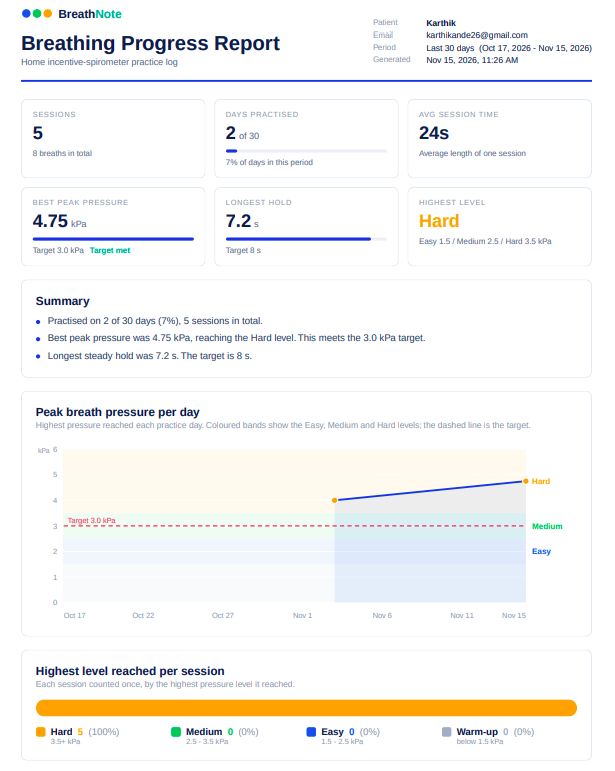
\includegraphics[width=0.95\linewidth]{figures/pdf_report_page1.png}}
  \end{minipage}\hspace{1.5em}
  \begin{minipage}[t]{0.44\linewidth}
    \vspace{0pt}\centering
    \fbox{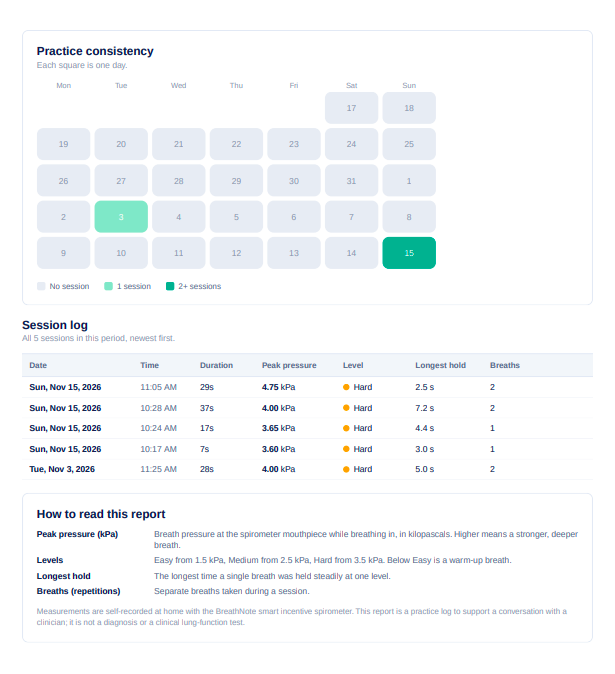
\includegraphics[width=0.95\linewidth]{figures/pdf_report_page2.png}}
  \end{minipage}
  \caption{A real progress report downloaded from BreathNote (last 30 days). Left: summary tiles, highlights, the daily peak-pressure chart and the levels reached. Right: the practice-consistency calendar, the session log and a guide on how to read the report.}
  \label{fig:pdfreport}
\end{figure}

\FloatBarrier
% =====================================================================
\section{The Sensor: HX710B Air Pressure Sensor Module}
\label{sec:sensor}

\subsection{What the sensor is}
The sensor we used is the \textbf{HX710B air pressure sensor module}, taken from the ECE store (catalogue ID 2026376, store location 52135). It is a small board of about \textbf{19.6\,mm $\times$ 13.5\,mm} with two parts:
\begin{enumerate}
  \item \textbf{MPS20N0040D pressure sensor:} a small metal-and-plastic package with a \textbf{nozzle}. Air pressure enters through the nozzle and acts on a tiny silicon diaphragm inside.
  \item \textbf{HX710B chip:} a 24-bit analog-to-digital converter (ADC) with a built-in amplifier. It turns the sensor's tiny voltage into a digital number.
\end{enumerate}

\begin{figure}[H]
\centering
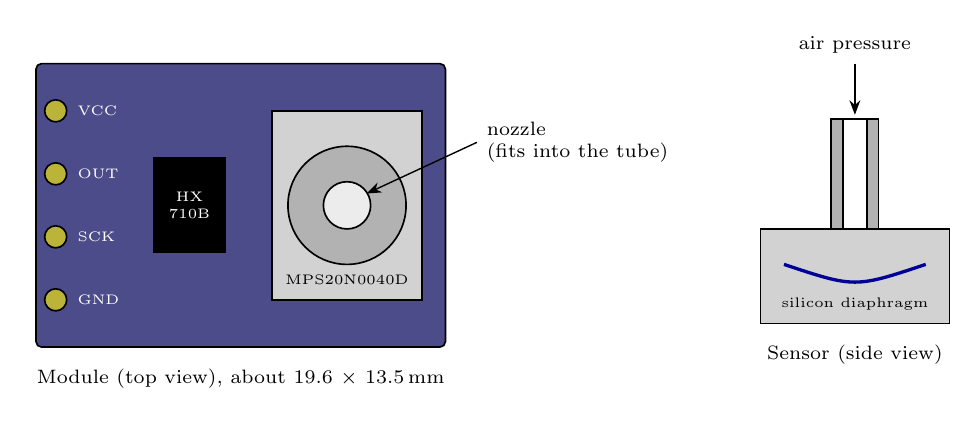
\begin{tikzpicture}[line width=0.6pt]
  % --- Board drawing (left) ---
  \begin{scope}
    \draw[fill=blue!35!black!70, rounded corners=2pt] (0,0) rectangle (5.2,3.6);
    \foreach \y in {0.6,1.4,2.2,3.0} \draw[fill=yellow!70!black] (0.25,\y) circle (0.14);
    \node[font=\tiny, white, right] at (0.4,3.0) {VCC};
    \node[font=\tiny, white, right] at (0.4,2.2) {OUT};
    \node[font=\tiny, white, right] at (0.4,1.4) {SCK};
    \node[font=\tiny, white, right] at (0.4,0.6) {GND};
    \draw[fill=black] (1.5,1.2) rectangle (2.4,2.4);
    \node[font=\tiny, white, align=center] at (1.95,1.8) {HX\\710B};
    \draw[fill=gray!35] (3.0,0.6) rectangle (4.9,3.0);
    \draw[fill=gray!60] (3.95,1.8) circle (0.75);
    \draw[fill=gray!15] (3.95,1.8) circle (0.3);
    \node[font=\tiny, align=center] at (3.95,0.85) {MPS20N0040D};
    \node[font=\scriptsize, align=center] at (2.6,-0.4) {Module (top view), about 19.6 $\times$ 13.5\,mm};
    \draw[-{Stealth}, line width=0.5pt] (5.6,2.6) node[right, font=\scriptsize, align=left]{nozzle\\(fits into the tube)} -- (4.2,1.95);
  \end{scope}
  % --- Side view of sensor (right) ---
  \begin{scope}[xshift=9.2cm, yshift=0.3cm]
    \draw[fill=gray!35] (0,0) rectangle (2.4,1.2);
    \draw[fill=gray!60] (0.9,1.2) rectangle (1.5,2.6);
    \draw[fill=white] (1.05,1.2) rectangle (1.35,2.6);
    \draw[line width=1.2pt, blue!60!black] (0.3,0.75).. controls (1.2,0.45).. (2.1,0.75);
    \node[font=\tiny, align=center] at (1.2,0.25) {silicon diaphragm};
    \draw[-{Stealth}, line width=0.5pt] (1.2,3.3) node[above, font=\scriptsize]{air pressure} -- (1.2,2.65);
    \node[font=\scriptsize] at (1.2,-0.4) {Sensor (side view)};
  \end{scope}
\end{tikzpicture}
\caption{Drawing of the HX710B air pressure sensor module (left) and the inside of the pressure sensor (right). Air enters the nozzle and bends a thin silicon diaphragm.}
\label{fig:hx710b}
\end{figure}

\subsection{Specifications}

\begin{table}[H]
\centering
\caption{Key specifications of the HX710B module (approximate, from vendor listings).}
\label{tab:sensorspec}
\small
\begin{tabularx}{0.85\linewidth}{@{}P{4.0cm} L@{}}
\toprule
\textbf{Property} & \textbf{Value} \\
\midrule
Pressure range  & 0--40\,kPa \\
Resolution      & 24-bit (very fine steps) \\
Supply voltage  & 3.3--5\,V (powered by the Arduino) \\
Board size      & About 19.6\,mm $\times$ 13.5\,mm \\
Cost            & About \rupee 150--250 \\
\bottomrule
\end{tabularx}
\end{table}

\textbf{Why it suits our use.} Our three levels need only \textbf{1.5, 2.5 and 3.5\,kPa}, which is well inside the sensor's 0--40\,kPa range. So the sensor never reaches its limit, and its 24-bit resolution picks up even gentle breaths from weak patients.

\subsection{Working principle}
\label{sec:sensor-principle}
Inside the sensor is a thin silicon diaphragm with tiny resistors on it. When the patient breathes, the air pressure bends the diaphragm and changes the resistance, which gives a very small voltage. The HX710B chip amplifies this voltage and converts it into a 24-bit number that the Arduino reads.

\begin{figure}[H]
\centering
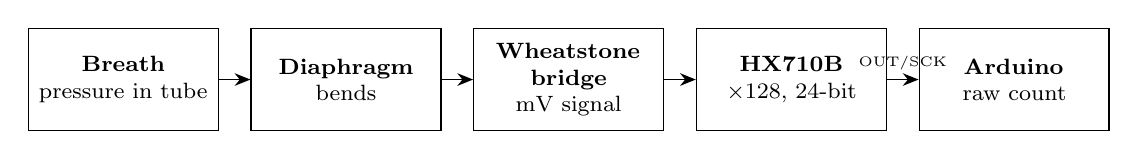
\begin{tikzpicture}[
    node distance=4mm,
    box/.style={draw=black, fill=white, line width=0.5pt, align=center,
                text width=2.2cm, minimum height=13mm, inner sep=3pt, font=\footnotesize},
    arr/.style={-{Stealth[length=2mm, width=1.6mm]}, line width=0.6pt}]
  \node[box] (a) {\textbf{Breath}\\ pressure in tube};
  \node[box, right=of a] (b) {\textbf{Diaphragm}\\ bends};
  \node[box, right=of b] (c) {\textbf{Wheatstone bridge}\\ mV signal};
  \node[box, right=of c] (d) {\textbf{HX710B}\\ $\times$128, 24-bit};
  \node[box, right=of d] (e) {\textbf{Arduino}\\ raw count};
  \draw[arr] (a)--(b); \draw[arr] (b)--(c); \draw[arr] (c)--(d); \draw[arr] (d)--node[above,font=\tiny]{OUT/SCK}(e);
\end{tikzpicture}
\caption{Signal chain inside the sensor module.}
\label{fig:sensorchain}
\end{figure}

\subsection{How we used this sensor}
\begin{itemize}
  \item We made a small hole in the spirometer tube, pushed the sensor nozzle into it and sealed the joint airtight.
  \item The tube's far end is closed by the spirometer body, so the pressure is the same along the tube, and the single sensor reads the breathing pressure of the whole tube.
  \item The Arduino reads the 24-bit raw value continuously and sends it over USB.
  \item The bridge converts raw values to kPa (Section~\ref{sec:calibration}) and streams them to the browser, where they drive the balls, the music and the repetition counter.
  \item Pressure above zero means breathing out into the closed tube, and below zero means breathing in. The application uses the size of the pressure, so the device works for both.
\end{itemize}

\subsection{Other approaches we tried, and why we did not use them}
\label{sec:alternatives}

We tried four approaches before choosing our final design.

\begin{figure}[H]
  \centering
  \begin{minipage}[c]{0.30\linewidth}
    \centering
    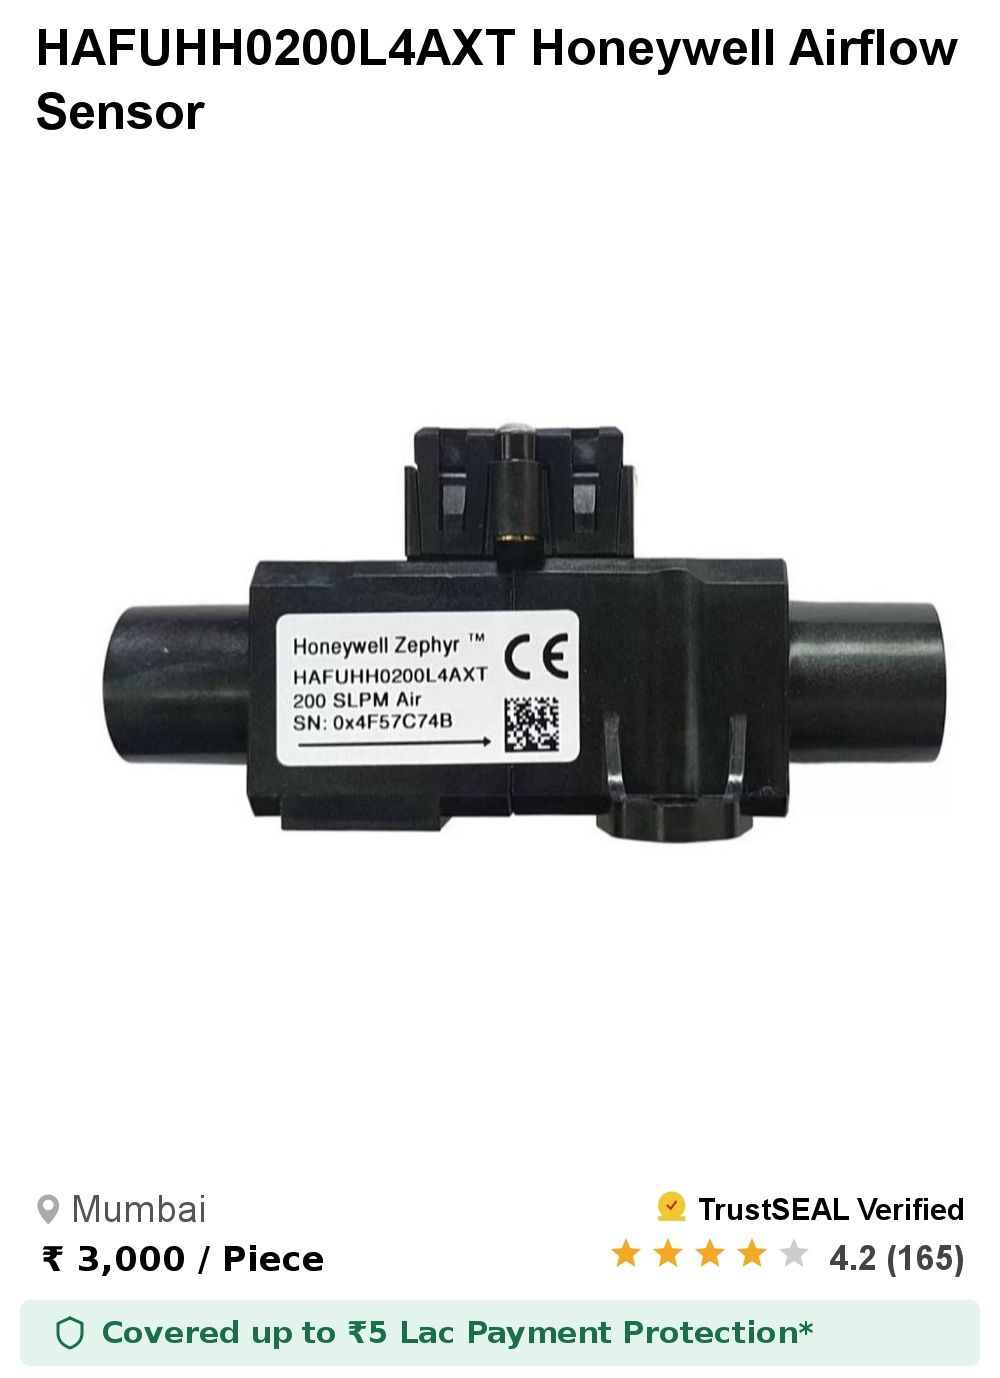
\includegraphics[width=\linewidth, height=3.2cm, keepaspectratio]{figures/honeywell.png}
  \end{minipage}\hfill
  \begin{minipage}[c]{0.66\linewidth}
    \textbf{Approach 1: Commercial airflow sensors (not used)}\par\smallskip
    Medical-grade airflow and pressure sensors from Honeywell and Sensirion, used in real ventilators and spirometers. They are accurate, but the affordable models were out of stock and the available ones cost more than \rupee 7,000, beyond our budget.
  \end{minipage}
  \caption{Commercial airflow sensors.}
  \label{fig:appr1}
\end{figure}

\begin{figure}[H]
  \centering
  \begin{minipage}[c]{0.30\linewidth}
    \centering
    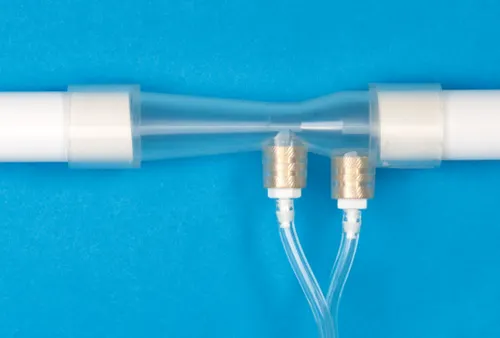
\includegraphics[width=\linewidth, height=3.2cm, keepaspectratio]{figures/venturi.png}
  \end{minipage}\hfill
  \begin{minipage}[c]{0.66\linewidth}
    \textbf{Approach 2: Venturi tube with two pressure sensors (not used)}\par\smallskip
    A tube with a narrow middle section, where faster air causes a pressure drop that gives the airflow. Gentle breathing created a pressure difference too small for low-cost sensors to measure reliably.
  \end{minipage}
  \caption{Venturi tube with two pressure sensors.}
  \label{fig:appr2}
\end{figure}

\begin{figure}[H]
  \centering
  \begin{minipage}[c]{0.30\linewidth}
    \centering
    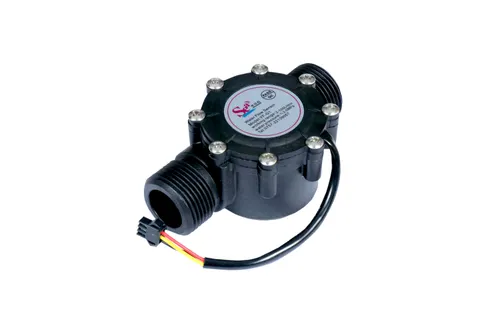
\includegraphics[width=\linewidth, height=3.2cm, keepaspectratio]{figures/turbine.png}
  \end{minipage}\hfill
  \begin{minipage}[c]{0.66\linewidth}
    \textbf{Approach 3: Turbine flow sensor (not used)}\par\smallskip
    A small fan that spins when air passes through it. The fan needs a strong airflow to start turning and was inaccurate at low flow, so it does not suit patients with weak breathing.
  \end{minipage}
  \caption{Turbine flow sensor.}
  \label{fig:appr3}
\end{figure}

\begin{figure}[H]
  \centering
  \begin{minipage}[c]{0.30\linewidth}
    \centering
    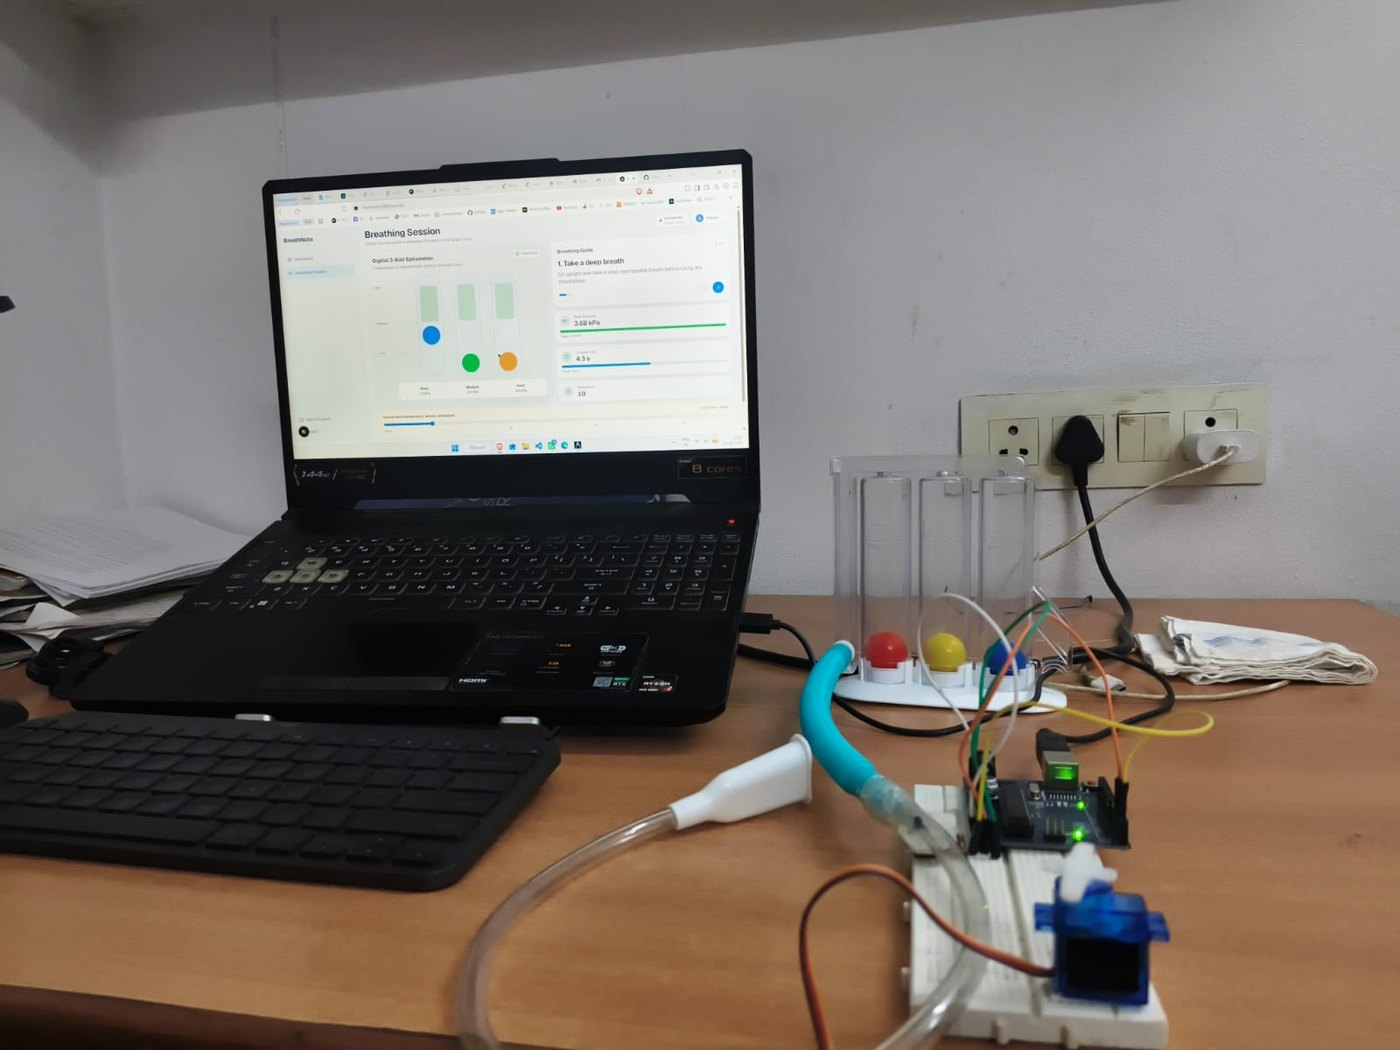
\includegraphics[width=\linewidth, height=3.2cm, keepaspectratio]{figures/prototype.jpg}
  \end{minipage}\hfill
  \begin{minipage}[c]{0.66\linewidth}
    \textbf{Approach 4: One pressure sensor in a closed tube (chosen)}\par\smallskip
    The spirometer body closes the far end of the tube, so each breath changes the pressure along the whole tube and one HX710B sensor is enough. It is cheap, was available immediately and works even with gentle breaths.
  \end{minipage}
  \caption{One pressure sensor in a closed tube.}
  \label{fig:appr4}
\end{figure}

\subsection{Calibration: How We Calibrate the Sensor Data and Use It}
\label{sec:calibration}

Calibration makes the sensor's numbers match the real breathing effort. We do it in three simple steps:

\begin{enumerate}[itemsep=4pt]
  \item \textbf{Find the zero.} Each time the system starts, the patient does not breathe for 3 seconds. The middle value of these readings becomes the ``zero'' level.
  \item \textbf{Convert to kPa.} Every reading is then turned into a pressure value in kPa using a scale factor, which can be adjusted if the balls move too easily or too slowly.
  \item \textbf{Match the real balls.} We breathed through the real 3-ball spirometer many times and noted the sensor reading each time a ball rose. From these trials we set the three levels: \textbf{Easy 1.5\,kPa, Medium 2.5\,kPa and Hard 3.5\,kPa}.
\end{enumerate}

\textbf{How we use the calibrated values.} The pressure moves the three virtual balls, controls the music, counts each breath (above 0.5\,kPa) and is saved in the database for the dashboard and reports.

\textbf{Note:} these levels are prototype values for testing. Final clinical targets will be set with doctors during a hospital pilot.

% =====================================================================
\section{Why Music Is Needed for Breathing Exercises}
\label{sec:whymusic}

The incentive spirometer works only if the patient uses it \textbf{often and correctly}, about 10 deep breaths every waking hour. But the exercise is boring, gives no reward and gives no feedback, so many patients skip it or do it wrongly. Music solves these problems.

\Needspace{6\baselineskip}
\subsection{What research says}
\begin{itemize}
  \item Music makes exercise \textbf{feel better and easier} and improves performance (review of 139 studies).
  \item Lung patients (COPD) who walked with music felt \textbf{less breathless} and walked farther.
  \item Music \textbf{reduces anxiety and pain} in patients after surgery \cite{kuhlmann}.
  \item Music changes breathing only when it \textbf{follows the breath}; background music has no effect \cite{bhandari}.
\end{itemize}

\Needspace{6\baselineskip}
\subsection{Why we added music to BreathNote}
\begin{itemize}
  \item \textbf{Enjoyable:} turns a boring, repeated exercise into a pleasant one.
  \item \textbf{Motivating:} each good breath is rewarded with music, so the patient wants to do more \cite{salimpoor}.
  \item \textbf{Instant feedback:} the sound tells the patient right away how well they are breathing.
  \item \textbf{Teaches the right technique:} the music grows only with slow, deep, held breaths.
  \item \textbf{Calming:} pleasant music lowers anxiety and stress \cite{dewitte}.
  \item \textbf{Active participation:} the patient's own breath plays the music, which keeps them engaged.
  \item \textbf{Familiar:} Indian swaras feel natural and calming to Indian patients.
\end{itemize}

\Needspace{6\baselineskip}
\subsection{Why music and not beeps or a screen?}
\begin{itemize}
  \item Beeps quickly become boring and annoying \cite{bhandari}.
  \item A screen must be watched all the time; music can be followed just by listening.
  \item Music carries emotion: it feels happy, calm and rewarding.
\end{itemize}

% =====================================================================
\section{Music in BreathNote}
\label{sec:music}

This section explains the music used in BreathNote: what swaras, harmony and chords are, which swaras we use, the order in which they are played, the smooth glide between them, and how the music is produced.

\subsection{Swaras: the notes of Indian music}
\label{sec:swaras}

In Indian classical music, a note is called a \textbf{swara}. There are seven basic swaras:
\begin{center}
\textbf{Sa \quad Ri \quad Ga \quad Ma \quad Pa \quad Dha \quad Ni \quad (\Sah)}
\end{center}
BreathNote plays three notes: \textbf{Ga}, \textbf{Pa} and the upper Sa (\Sah). The middle \textbf{Sa} is not played; it is the reference pitch from which these three notes are calculated. Each ratio to Sa is tuned in \emph{just intonation}, the natural tuning used by a tanpura and by singers (Table~\ref{tab:freq}). The following parts explain each of these notes and why we used it.

\begin{table}[H]
\centering
\caption{The swaras used in BreathNote (Sa = 261.63\,Hz, as set in \texttt{levels.yaml}).}
\label{tab:freq}
\small
\begin{tabular}{@{}l l c r l@{}}
\toprule
\textbf{Swara} & \textbf{Full name} & \textbf{Ratio to Sa} & \textbf{Frequency} & \textbf{Role in BreathNote} \\
\midrule
Sa   & Shadja (middle octave) & 1     & 261.63\,Hz & Reference pitch only (not played) \\
Ga   & Antara Gandhara (G3)   & 5/4   & 327.04\,Hz & Reached by ball 1 (Easy) \\
Pa   & Panchama               & 3/2   & 392.45\,Hz & Reached by ball 2 (Medium) \\
\Sah & Tara Shadja (upper Sa) & 2     & 523.26\,Hz & Reached by ball 3 (Hard) \\
\bottomrule
\end{tabular}
\end{table}

\Needspace{9\baselineskip}
\subsubsection{Sa: the base note (Shadja)}
\textbf{What is Sa?}
\begin{itemize}
  \item Sa is the first of the seven swaras: Sa, Ri, Ga, Ma, Pa, Dha and Ni.
  \item Its full name, \emph{Shadja}, comes from \emph{shad} (six) and \emph{ja} (born): \textbf{the note that gives birth to the other six}.
  \item It is the \textbf{foundation and reference point} of Indian music. Every other swara is defined by its distance from Sa, so a note is heard as Ga or Pa only in relation to Sa.
  \item Sa is a \textbf{fixed note}: it has no higher or lower forms and is sung without ornamentation.
\end{itemize}

\Needspace{5\baselineskip}
\textbf{Sa in Indian music vs Western music}
\begin{itemize}
  \item \textbf{Western music:} each note has a fixed frequency. For example, the note A is always 440\,Hz.
  \item \textbf{Indian music:} notes are \textbf{relative to Sa}. Each singer chooses the Sa that suits their voice, and all the other notes move with it.
\end{itemize}

\Needspace{5\baselineskip}
\textbf{Why we used Sa in BreathNote}
\begin{itemize}
  \item \textbf{Sa as the reference pitch:} in BreathNote, Sa is \textbf{not played}. It is the reference from which every played note is calculated: Ga is 5/4 of Sa, Pa is 3/2 of Sa and the upper Sa is 2 times Sa, exactly as a singer tunes every swara from their own Sa.
  \item \textbf{Sa returns as the final note:} the only Sa the patient hears is the upper Sa (\Sah), one octave higher, at the top of the exercise.
  \item \textbf{Sa is a setting, not fixed:} because Indian pitch is relative, Sa is stored as a setting (now 261.63\,Hz, the note C4). Ga, Pa and the upper Sa are always calculated from it, so if Sa is changed, all the notes move together and stay in tune.
\end{itemize}

\Needspace{5\baselineskip}
\textbf{How this helps the patient}
\begin{itemize}
  \item Because every note is calculated from the same Sa, the notes always fit together and stay \textbf{in tune}, so the music feels stable and calm instead of random.
  \item The pitch can be set to whatever the patient finds most \textbf{comfortable}, just as a singer chooses their own Sa.
\end{itemize}

\Needspace{9\baselineskip}
\subsubsection{Sa and Pa: the fixed notes}
\textbf{What makes Sa and Pa special?}
\begin{itemize}
  \item Five swaras (Ri, Ga, Ma, Dha and Ni) can each be sung in two or three positions, which gives ragas their different characters.
  \item \textbf{Sa and Pa never change.} They are called fixed (\emph{achala} or \emph{prakriti}) swaras, and every raga uses the same Sa and the same Pa.
  \item Because they have no variants, they act as \textbf{base positions}. This is why the 12 pitch positions in an octave are counted as $2 + (5 \times 2) = 12$.
  \item Sa and Pa are sung \textbf{without ornamentation} (gamaka), because they are stable notes.
\end{itemize}

\Needspace{5\baselineskip}
\textbf{Sa and Pa in practice}
\begin{itemize}
  \item Musicians practise \textbf{Sa--Pa--Sa daily} to set and hold the correct pitch and to train the ear.
  \item \textbf{Sa and Pa together are the best consonant pair}: the most pleasant and stable combination of two notes.
\end{itemize}

\Needspace{5\baselineskip}
\textbf{Why we used Pa in BreathNote}
\begin{itemize}
  \item Pa is the target of the \textbf{second (green) ball}, the Medium level.
  \item It is tuned exactly to \textbf{3/2 of Sa} (392.45\,Hz).
  \item When this ball reaches the top, Pa is held, and together with the held Ga it forms a steady, consonant two-note harmony (\textbf{Ga\,+\,Pa}).
\end{itemize}

\Needspace{5\baselineskip}
\textbf{How this helps the patient}
\begin{itemize}
  \item Pa is a fixed, stable note, so it sounds \textbf{open, steady and grounding}, without strong emotion.
  \item This suits a patient who may be tired, in pain or anxious.
\end{itemize}

\Needspace{9\baselineskip}
\subsubsection{The forms of Ga and our Antara Gandhara (G3)}
\textbf{The forms of Ga}
\begin{itemize}
  \item Ga (Gandhara) is the third swara. Unlike Sa and Pa, it can be sung in different positions:
  \begin{itemize}
    \item \textbf{G1 -- Shuddha Gandhara} (lowest);
    \item \textbf{G2 -- Sadharana Gandhara} (middle);
    \item \textbf{G3 -- Antara Gandhara} (highest).
  \end{itemize}
  \item A \emph{swarasthana} is the fixed pitch position of a swara. There are 12 distinct positions, but Carnatic music gives them 16 names, because some positions share a name (for example R2 = G1).
  \item Choosing a different position of a swara \textbf{changes the character of the raga}.
\end{itemize}

\Needspace{5\baselineskip}
\textbf{Why we used G3 in BreathNote}
\begin{itemize}
  \item Our Ga is \textbf{Antara Gandhara (G3)}, tuned to exactly \textbf{5/4 of Sa} (327.04\,Hz), the way a tanpura player tunes it by ear.
  \item It is the target of the \textbf{first (blue) ball}, the Easy level.
  \item When the breath is still weak, the sound is soft breath noise; as the first ball rises, the noise slowly focuses into a clear G3.
\end{itemize}

\Needspace{5\baselineskip}
\textbf{How this helps the patient}
\begin{itemize}
  \item G3 is the Ga of bright, happy ragas such as Mohanam and Sankarabharanam.
  \item As the very first clear note the patient hears, it gives an \textbf{immediate, positive and encouraging} reward.
\end{itemize}

\Needspace{9\baselineskip}
\subsubsection{Octave: the upper Sa}
\textbf{What is an octave?}
\begin{itemize}
  \item An octave is the distance from one Sa to the next Sa above it.
  \item The higher Sa has \textbf{exactly double} the frequency of the lower Sa, which is why the ear hears it as ``the same note, only higher''.
  \item If Sa is $f$, the higher Sa is $2f$ and the lower Sa is $f/2$.
\end{itemize}

\Needspace{5\baselineskip}
\textbf{The three octaves in Indian music}
\begin{itemize}
  \item \textbf{Mandra} -- the low octave;
  \item \textbf{Madhya} -- the middle octave;
  \item \textbf{Tara} -- the high octave. The higher Sa is written with a dot above it (\.{S}); in this report we write it as \Sah.
\end{itemize}

\Needspace{5\baselineskip}
\textbf{Why we used the upper Sa in BreathNote}
\begin{itemize}
  \item The \textbf{third (orange) ball}, the Hard level, takes the pitch from Pa up to the upper Sa in the Tara octave.
  \item Its frequency is $2 \times 261.63 = 523.26$\,Hz.
  \item It is the highest note of the exercise and is reached only by the deepest, strongest breath.
\end{itemize}

\Needspace{5\baselineskip}
\textbf{How this helps the patient}
\begin{itemize}
  \item At the last ball, the patient does not hear the upper Sa alone. Ga and Pa are still sounding, so the upper Sa is added on top of them and \textbf{completes the full chord Ga\,+\,Pa\,+\,\Sah}.
  \item The upper Sa closes the chord at the octave, so the music sounds \textbf{full and complete}. This gives the hardest goal, the deepest and longest breath, the richest and most satisfying reward.
\end{itemize}

\subsection{What are harmony and chords?}
\label{sec:harmony}

Music can be built in two basic ways: by placing notes \emph{one after another}, or by sounding them \emph{together}. These two ways are called melody and harmony.

\Needspace{5\baselineskip}
\textbf{Melody.}
\begin{itemize}
  \item A \textbf{melody} is a series of notes played \textbf{one after another}, in time. It is the part of the music we can sing or hum, the ``tune'' of a song.
  \item Only one note sounds at any moment; the ear follows the notes as they move up and down.
  \item \textbf{Example:} singing Sa, then Ga, then Pa, then the upper Sa, one note at a time, is a melody.
  \item Indian classical music is mainly built on melody: a single, richly ornamented line of swaras.
\end{itemize}

\Needspace{5\baselineskip}
\textbf{Harmony.}
\begin{itemize}
  \item \textbf{Harmony} is when two or more \textbf{different} notes sound \textbf{at the same time}.
  \item The notes do not take turns; they mix together, and the ear hears them as \textbf{one combined sound}.
  \item \textbf{Example:} playing Sa and Pa together creates a harmony. Each note can still be heard, but together they make a fuller and richer sound than either note alone.
  \item A simple way to picture it: a melody is like a single line drawn across a page, while harmony is like several lines stacked on top of each other at the same moment.
\end{itemize}

\Needspace{5\baselineskip}
\textbf{Chord.}
\begin{itemize}
  \item A \textbf{chord} is a special kind of harmony: a group of \textbf{three or more} different notes sounding together.
  \item Two notes together make a simple harmony (called an interval); three or more notes together make a chord, which sounds even fuller and more complete.
  \item \textbf{Example:} Ga, Pa and the upper Sa sounding together form a chord. This is exactly the chord BreathNote builds at the deepest breath.
  \item Chords are the foundation of Western music, where songs are built on sequences of chords.
\end{itemize}

When two notes sound together and the ear hears them as smooth, pleasant and restful, they are called \textbf{consonant}. The reason is simple:
\begin{itemize}
  \item Every musical note is not a single frequency. It also contains \textbf{overtones} (harmonics) at 2, 3, 4, 5, \ldots{} times its frequency.
  \item When two notes have a \textbf{simple frequency ratio}, like 2:1, 3:2 or 5:4, many of their overtones \emph{line up exactly}. The ear hears a smooth, single, blended sound.
\end{itemize}
Studies show that people prefer chords whose notes fit together as one harmonic series, and that the brain responds more strongly and cleanly to consonant intervals.

\textbf{The ratios of the notes in BreathNote}
\begin{table}[H]
\centering
\small
\begin{tabular}{@{}l c l@{}}
\toprule
\textbf{Notes together} & \textbf{Frequency ratio} & \textbf{How it sounds} \\
\midrule
Ga and Pa                  & 6: 5 & Consonant; soft and warm \\
Pa and upper Sa            & 4: 3 & Consonant; stable \\
Ga and upper Sa            & 8: 5 & Consonant; sweet \\
\bottomrule
\end{tabular}
\end{table}
\begin{itemize}
  \item These are the pairs that actually sound together in BreathNote. Because Ga, Pa and \Sah{} are all tuned from the same Sa (5/4, 3/2 and 2), every pair has a \textbf{simple ratio}, so every combination is consonant.
  \item By contrast, Ri would sit very close below Ga (a ratio of 10:9), so its vibrations would clash with Ga and give a rough sound. This is one reason we did not use Ri.
\end{itemize}

\textbf{Harmony in Indian music.} Carnatic music is mainly melodic; it does not use chords the way Western music does. But harmony is always present: the \textbf{tanpura drone} plays Sa and Pa continuously, and every swara is sung \emph{against} this drone. Musicians tune by listening for the swara to ``lock'' with the drone, which is exactly the consonance described above. The tanpura's special bridge (\emph{jivari}) brings out its overtones so strongly that musicians can hear a Ga sounding inside the drone by itself, often called the \emph{swayambhu} (self-born) gandharam. BreathNote uses the same tuning idea: Ga, Pa and \Sah{} are tuned exactly from Sa, so they lock together the way swaras lock with a tanpura. To keep the sound simple and clear, Sa itself is not played; it is used only as the reference pitch.

\textbf{The chord we build.} Ga, Pa and \Sah{} are, in Western terms, the three notes of a \textbf{major chord} (in C major: E, G and C). It is one of the most stable and consonant chords in music.

\Needspace{5\baselineskip}
\textbf{How BreathNote builds a harmony}
\begin{itemize}
  \item In most music feedback, one note replaces the next. In BreathNote, when a ball reaches the top, its note \textbf{keeps sounding}, and the next note is added on top:
  \begin{enumerate}
    \item \textbf{Blue ball at the top:} Ga sounds on its own.
    \item \textbf{Green ball rising:} a second voice glides up from Ga towards Pa, while a held Ga stays behind. At the top, the patient hears \textbf{Ga\,+\,Pa} together.
    \item \textbf{Orange ball rising:} the voice glides up from Pa to the upper Sa, while Ga and Pa both stay. At the top, the patient hears the full chord \textbf{Ga\,+\,Pa\,+\,\Sah}.
  \end{enumerate}
  \item Each held note fades in smoothly just as the gliding voice starts to leave it, so it sounds as if \textbf{one voice splits into two, and then three}.
  \item The held notes are played slightly softer than the gliding voice, so the moving note stays clearly in front.
  \item If the breath weakens, the balls fall and the top notes fade away in reverse order, so the chord \textbf{breaks} as soon as the effort drops.
\end{itemize}
\begin{itemize}
  \item In this way, BreathNote uses all three ideas together: a \textbf{melody} that follows the breath, a \textbf{harmony} that builds up as each level is reached, and a full \textbf{chord} as the final reward.
\end{itemize}

\subsection{Which swaras we used}
\label{sec:whichswaras}

The swaras we use are:
\begin{itemize}
  \item \textbf{Ga}, \textbf{Pa} and \textbf{\Sah} as the three notes reached by the three balls.
\end{itemize}

\begin{table}[H]
\centering
\caption{What the patient hears at each stage of a breath.}
\label{tab:musicmap}
\small
\begin{tabularx}{\linewidth}{@{}P{2.6cm} P{2.6cm} L@{}}
\toprule
\textbf{Ball (level)} & \textbf{Pressure band} & \textbf{Sound} \\
\midrule
At rest            & below about 0.05\,kPa   & Silence \\
Ball 1 (blue, Easy)& 0 -- 1.5\,kPa       & Soft breath noise slowly focuses into a clear \textbf{Ga} \\
Ball 2 (green, Medium) & 1.5 -- 2.5\,kPa & \textbf{Ga stays}; a second voice glides smoothly up from Ga to \textbf{Pa} $\Rightarrow$ \textbf{Ga\,+\,Pa} \\
Ball 3 (orange, Hard)  & 2.5 -- 3.5\,kPa & \textbf{Ga and Pa stay}; the voice glides from Pa up to \textbf{\Sah} $\Rightarrow$ \textbf{Ga\,+\,Pa\,+\,\Sah} \\
Effort drops       & falls back         & Notes fade in reverse as balls fall; silence at rest \\
\bottomrule
\end{tabularx}
\end{table}

\begin{figure}[H]
\centering
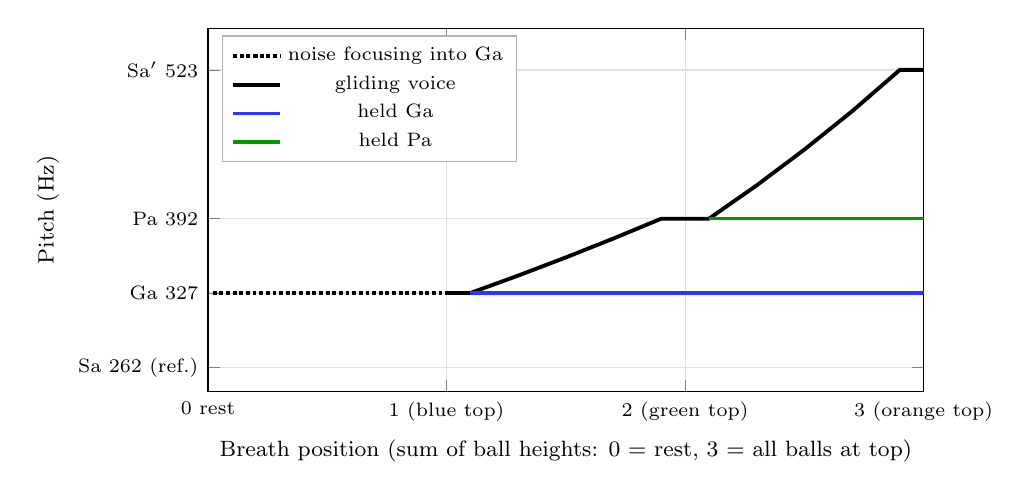
\begin{tikzpicture}
\begin{axis}[
    width=0.88\linewidth, height=6.2cm,
    xmin=0, xmax=3, ymin=240, ymax=560,
    xlabel={Breath position (sum of ball heights: 0 = rest, 3 = all balls at top)},
    ylabel={Pitch (Hz)},
    xtick={0,1,2,3}, xticklabels={0 rest, 1 (blue top), 2 (green top), 3 (orange top)},
    ytick={261.63,327.04,392.45,523.26},
    yticklabels={Sa 262 (ref.), Ga 327, Pa 392, \Sah{} 523},
    tick label style={font=\scriptsize}, label style={font=\footnotesize},
    grid=major, grid style={black!12},
    legend style={font=\scriptsize, at={(0.02,0.98)}, anchor=north west, draw=black!30}]
  \addplot[black, line width=1.4pt, densely dotted] coordinates {(0.02,327.04) (1,327.04)};
  \addlegendentry{noise focusing into Ga}
  \addplot[black, line width=1.4pt] coordinates {(1,327.04) (1.1,327.04) (1.3,342.3) (1.5,358.3) (1.7,375.0) (1.9,392.4) (2.1,392.4) (2.3,421.7) (2.5,453.2) (2.7,486.9) (2.9,523.3) (3,523.3)};
  \addlegendentry{gliding voice}
  \addplot[blue!80, line width=1.2pt] coordinates {(1.1,327.04) (3,327.04)};
  \addlegendentry{held Ga}
  \addplot[green!60!black, line width=1.2pt] coordinates {(2.1,392.45) (3,392.45)};
  \addlegendentry{held Pa}
\end{axis}
\end{tikzpicture}
\caption{The breath-driven swara glide, computed from our code. The gliding voice rises noise $\rightarrow$ Ga $\rightarrow$ Pa $\rightarrow$ \Sah{} on a musical (logarithmic) scale. Each note that is reached stays sounding, so the sound builds into Ga\,+\,Pa and then Ga\,+\,Pa\,+\,\Sah{}. Sa (262\,Hz) is shown only as the reference pitch; it is not played.}
\label{fig:glide}
\end{figure}

\subsection{Why this order: Ga, then Pa, then \Sah}
\label{sec:whyorder}

\begin{enumerate}
  \item \textbf{Rising effort, rising pitch.} Ga $<$ Pa $<$ \Sah{} in pitch. As the patient breathes harder and the balls go up, the music also goes up. People naturally connect higher pitch with ``higher'' and ``more'', so the mapping needs no explanation.
  \item \textbf{From open to complete.} Ga alone is a single bright note. Adding Pa makes a stable two-note harmony. Adding \Sah{} completes the chord Ga\,+\,Pa\,+\,\Sah, the notes of a major chord. The music moves from \emph{start} to \emph{stable} to \emph{complete}, like a small musical story on each breath, ending in resolution at Sa.
  \item \textbf{Why not start at Sa?} Sa is the reference pitch from which all the notes are calculated, and we chose not to play it. Starting at Ga gives a clearly bright, positive note as the first reward, and Sa returns only at the very top as \Sah, marking that the goal is complete.
  \item \textbf{From noise to note.} Below the first goal, the sound is breath noise that slowly focuses into Ga. Noise means ``not yet''; a clear note means ``achieved''. This follows music-biofeedback research, where noise mixed into music signalled incorrect breathing and clean music rewarded correct breathing \cite{bhandari}.
  \item \textbf{Smooth glides like gamakas.} The pitch glides continuously between swaras on a musical (logarithmic) scale, inspired by the gamakas of Carnatic music and by our earlier Gamaka Slider (Section~\ref{sec:gamaka}). Near the top of each ball the pitch holds the exact swara (10\% of the travel), so a breath held there is heard as a clean Ga, Pa or \Sah.
\end{enumerate}

\Needspace{9\baselineskip}
\subsection{Gamaka: the smooth glide between notes}
\label{sec:gamaka}
\textbf{What is a gamaka?}
\begin{itemize}
  \item Gamakas are the \textbf{ornaments} of Indian music.
  \item Instead of jumping straight from one note to the next, the voice moves with \textbf{smooth curves, slides and gentle oscillations}.
  \item Gamakas make the change between notes smooth and expressive, and give each raga its special character; a raga is incomplete without them.
  \item Carnatic music uses heavier ornamentation than Hindustani music. Sa and Pa are sung without gamakas, because they are fixed notes.
\end{itemize}

\Needspace{5\baselineskip}
\textbf{How BreathNote uses a gamaka-like glide}
\begin{itemize}
  \item Our pitch \textbf{never jumps}; it \textbf{glides smoothly} from Ga up to Pa with the second ball, and from Pa up to \Sah{} with the third.
  \item The glide follows a musical (logarithmic) scale, so equal increases in breath sound like equal musical steps.
  \item It is inspired by the gamaka and by our earlier \textbf{Gamaka Slider} exercise in this course.
  \item As with Sa and Pa in music, the target notes themselves are held \textbf{steady} near the top of each ball, without wobbling.
\end{itemize}

\Needspace{5\baselineskip}
\textbf{How this helps the patient}
\begin{itemize}
  \item The smooth glide follows the slow, steady breath naturally, so the patient \textbf{hears every small improvement} in effort.
  \item Sudden jumps would sound mechanical; the gamaka-like glide sounds musical and calming.
\end{itemize}

\subsection{How the music is produced (implementation)}
\label{sec:music-impl}

The music is created live in the web browser, using the browser's built-in sound system (the Web Audio API). No recorded audio files are used, so the sound responds instantly to the breath and works even without internet.
\begin{itemize}
  \item \textbf{It follows the balls:} as the three balls rise, the pitch glides smoothly from breath noise to Ga, then to Pa, then to the upper Sa.
  \item \textbf{Notes stay to build the harmony:} when a ball reaches the top, its note keeps playing, so Ga, then Ga\,+\,Pa, then Ga\,+\,Pa\,+\,\Sah{} are heard.
  \item \textbf{Sa is not played:} it is only the reference pitch from which Ga, Pa and the upper Sa are calculated.
  \item \textbf{Silent when not needed:} there is no sound when the balls are at rest, and the music stops when the session is paused or ended. A Sound on/off button lets the patient mute it.
  \item \textbf{Adjustable pitch:} the pitch of Sa is kept in a settings file, so it can be changed for each patient's comfort.
\end{itemize}

% =====================================================================
\section{Music and Health}
\label{sec:musicandhealth}

This section explains how music is linked to health, why we chose only Ga, Pa and \Sah, the health benefits of each of these swaras, why playing them together as a harmony helps the patient, and how BreathNote makes the patient an active part of the music.

\begin{figure}[H]
  \centering
  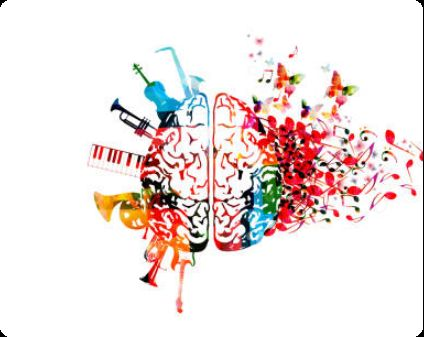
\includegraphics[height=4.4cm]{figures/music_brain.png}
  \caption{Music engages many parts of the brain: hearing, emotion, memory, reward and movement.}
  \label{fig:musicbrain}
\end{figure}

\Needspace{9\baselineskip}
\subsection{How music is related to health}
\label{sec:musichealth}
\textbf{Mental health.}
\begin{itemize}
  \item \textbf{Less stress and anxiety.} A large review of 104 randomised trials found that music interventions reduce both the physical signs of stress (heart rate, blood pressure, stress hormones) and the feeling of stress \cite{dewitte}.
  \item \textbf{Less anxiety and pain around surgery.} A review of 92 trials with more than 7,000 surgical patients found that music clearly reduced anxiety and pain \cite{kuhlmann}. A Cochrane review found that music before surgery reduces anxiety. Our users are mostly surgical patients, so this is directly relevant.
  \item \textbf{Reward and motivation.} Pleasant music releases \textbf{dopamine} in the brain's reward system, both while waiting for a musical peak and when it arrives \cite{salimpoor}. Dopamine is the chemical of motivation: it makes us want to do something again.
  \item \textbf{Mood.} Pleasant, consonant music activates brain areas linked to positive emotion; dissonant music activates areas linked to unpleasant feelings.
  \item \textbf{Attention.} Boredom lowers motivation; music holds attention and turns a repetitive action into an experience.
  \item \textbf{Makes repetitive actions engaging.} When the same action is repeated many times, such as an exercise, people quickly get bored and lose interest. Music makes the activity \textbf{engaging}: it reduces boredom, keeps the person interested, makes time feel shorter and helps them continue for longer. This is why music is widely used in physiotherapy, rehabilitation and exercise.
\end{itemize}

\Needspace{5\baselineskip}
\textbf{Physical health.}
\begin{itemize}
  \item \textbf{Breathing and heart.} Slow music and slow, regular breathing lower the breathing rate and heart rate. Slow breathing at about 6 breaths per minute increases heart-rate variability, a sign that the calming (parasympathetic) nervous system is active.
  \item \textbf{Biofeedback.} When music responds to the breath, people learn to slow down and control their breathing, even during a demanding task; music alone does not do this \cite{bhandari}.
  \item \textbf{Rehabilitation.} Rhythm and melody help repetitive physical therapy, for example walking after a stroke.
\end{itemize}

\textbf{How BreathNote uses this.} BreathNote uses music in three ways at once: as a \emph{reward} (the chord builds when the patient succeeds), as \emph{biofeedback} (the sound tells the patient, without looking, how strong and how steady the breath is), and as a \emph{calming sound} (calm, consonant notes) during an exercise that patients often find uncomfortable.

\subsection{Why only Ga, Pa and \Sah?}
\label{sec:whyonly}

\begin{enumerate}
  \item \textbf{Three balls, three notes.} The spirometer has three balls, so we need three clear goals. One note per ball makes the link between effort and sound easy to understand.
  \item \textbf{They are the most consonant notes with Sa.} Measured from the reference Sa, the three simplest ratios in music are 2:1 (\Sah), 3:2 (Pa) and 5:4 (Ga). Because all three come from the same Sa, they also sound smooth with each other (6:5, 4:3 and 8:5).
  \item \textbf{They are nature's own chord.} The overtones of Sa itself are Sa, \Sah, Pa, Sa, Ga, Pa, \ldots{}. So Ga, Pa and \Sah{} are already ``inside'' Sa. Playing them is like opening up the sound of Sa. This is why the ear accepts them so easily and why the tanpura seems to sing Ga by itself.
  \item \textbf{We avoided the tense notes.} Ri (9/8) sits very close to Ga, and Ni (15/8) sits very close below \Sah, so with our notes they would create roughness and a feeling that ``something must resolve''. Ma (4/3) pulls back towards Ga, and Dha changes the mood depending on the raga. For a calming exercise repeated a hundred times a day, we wanted only restful notes.
  \item \textbf{They are common to many ragas.} Sa, antara Ga and Pa appear together in many well-known ragas: Mohanam, Hamsadhwani, Shankarabharanam and Kalyani. So the sound feels familiar and pleasant, without belonging to only one raga or mood.
  \item \textbf{Easy to hear the difference.} Ga, Pa and \Sah{} are clearly spaced (a major third, then a minor third, then a fourth). A patient with no music training can still hear that the sound is ``going up'' and when it is ``complete''.
  \item \textbf{Chosen with our mentors.} We discussed the choice of swaras with our course mentor, Saroja Ma'am, and with Suswara.
\end{enumerate}

\Needspace{9\baselineskip}
\subsubsection{Bhopali and Shivaranjini: why our Ga is the bright Ga}
\textbf{Two ragas, one difference}
\begin{itemize}
  \item \textbf{Bhopali} (called \textbf{Mohanam} in Carnatic music): S R2 \textbf{G3} P D2 -- bright, happy and peaceful.
  \item \textbf{Shivaranjini}: S R2 \textbf{G2} P D2 -- dark, sad and full of longing.
  \item The \textbf{only difference is Ga}: the higher Ga (G3) makes the raga bright, and the lower Ga (G2) makes it sad.
\end{itemize}

\Needspace{5\baselineskip}
\textbf{One note decides the mood}
\begin{itemize}
  \item Shivaranjini is used for sad or dark emotions; the film composer Ilayaraja used it for such songs.
  \item Changing even one note gives a different raga with a different mood.
\end{itemize}

\Needspace{5\baselineskip}
\textbf{Why this mattered for BreathNote}
\begin{itemize}
  \item This example guided one of our most important decisions: \textbf{which Ga to use}.
  \item Since Ga decides whether the music sounds happy or sad, we deliberately chose the \textbf{higher Ga (G3)} of Bhopali/Mohanam, not G2.
\end{itemize}

\Needspace{5\baselineskip}
\textbf{How this helps the patient}
\begin{itemize}
  \item A patient recovering from surgery or lung illness needs encouragement, not sad music.
  \item The bright G3 makes every successful breath sound \textbf{positive and uplifting}, which supports mood and motivation.
\end{itemize}

\Needspace{9\baselineskip}
\subsubsection{Ganapati raga: our three notes form a real raga}
\textbf{What is the Ganapati raga?}
\begin{itemize}
  \item Most ragas use five, six or seven swaras. Ragas with only three or four swaras are very rare.
  \item The great Carnatic musician \textbf{M.~Balamuralikrishna} created the \textbf{Ganapati} raga, which uses only \textbf{three swaras: Sa, Ga and Pa}. It is used in the song ``Gam Ganapatim''.
\end{itemize}

\Needspace{5\baselineskip}
\textbf{What happens when a raga has only three swaras?}
\begin{itemize}
  \item \textbf{Every note stands out clearly.} With so few notes, each swara is heard distinctly, so the listener can easily follow the melody and recognise each note.
  \item \textbf{There are no clashing notes.} Sa, Ga and Pa are well spaced and blend smoothly with each other, so the music always sounds consonant, with no tense or rough moments.
  \item \textbf{The mood becomes simple and bright.} Sa, Ga and Pa together have a bright, auspicious and peaceful character, and nothing in the raga disturbs this mood.
  \item \textbf{Movement creates the variety.} Since there are so few notes, the beauty of the music comes from how the notes are joined: smooth glides between them, holding them, and moving to the higher Sa.
  \item \textbf{It is still a complete raga.} Even with only three notes, it sounds like real, finished music, which shows that a few well-chosen notes are enough.
\end{itemize}

\Needspace{5\baselineskip}
\textbf{How this applies to BreathNote}
\begin{itemize}
  \item BreathNote uses the \textbf{same three swaras}, Sa, Ga and Pa: Ga and Pa are played directly, and Sa is played in the upper octave (\Sah), while the middle Sa is the reference pitch. Our note set is therefore a real, accepted Carnatic note set, not a random choice.
  \item \textbf{One clear note for each ball:} because there are only a few notes, each ball has its own distinct note (Ga, Pa and \Sah). Any patient, even without musical training, can clearly hear when they move from one level to the next.
  \item \textbf{Always consonant:} since Sa, Ga and Pa never clash, every sound in the exercise, from a single note to the full chord, is pleasant and calm.
  \item \textbf{Variety from movement, not from more notes:} just as in the Ganapati raga, our music gets its richness from how the notes are joined: the smooth glide from Ga to Pa to \Sah, the holding of each note and the building harmony.
  \item \textbf{Simple enough to repeat:} the patient does this exercise more than a hundred times a day. A small, clear set of notes is easy to follow every time and never confusing.
\end{itemize}

\Needspace{5\baselineskip}
\textbf{How this helps the patient}
\begin{itemize}
  \item The patient hears a \textbf{proper, pleasant piece of Indian music}, even though only three notes are used.
  \item The clear, simple sound makes it easy to understand their own progress just by listening.
\end{itemize}

\subsection{Benefits of each swara for health}
\label{sec:benefits}

\subsubsection{Ga (antara gandharam, major third, 5:4)}
\begin{itemize}
  \item \textbf{Mood:} Ga is the note that makes a sound ``bright'' and ``happy''. The major third is the key difference between major (bright) and minor (sad) music, and it is linked with positive, cheerful emotion in listeners. Ragas built on antara gandharam, such as Mohanam and Shankarabharanam, are traditionally described as joyful and auspicious.
  \item \textbf{Stress:} because it is tuned in a simple ratio from Sa and blends smoothly with Pa, Ga sounds restful, not tense. Consonant sounds activate brain regions linked to pleasure rather than discomfort.
  \item \textbf{Role in BreathNote:} Ga is the \emph{first reward}. The moment the noise turns into a clear Ga, the patient knows the first goal is reached. This early success builds confidence and encourages the patient to continue.
  \item \textbf{Physical:} holding a steady Ga needs a steady breath, which trains slow, controlled breathing; slow breathing lowers heart rate and calms the nervous system.
\end{itemize}

\subsubsection{Pa (panchamam, perfect fifth, 3:2)}
\begin{itemize}
  \item \textbf{Stability and calm:} after the octave, the fifth is the most consonant interval in all music. Pa is a fixed (achala) note, the ``pillar'' of the scale. Together with Sa, it forms the drone of the tanpura, which musicians and meditators use for centering and calm.
  \item \textbf{Grounding:} the Sa--Pa sound is open and steady. It gives a sense of balance and support without strong emotion, which suits patients in pain or anxiety.
  \item \textbf{Role in BreathNote:} reaching Pa (while Ga is still sounding) means the patient has reached the medium level. The sound changes from a single note to a two-note harmony: a clear sign of progress.
  \item \textbf{Physical:} to keep the Pa sounding, the patient must hold a stronger breath. This is the sustained deep breath that opens the lower lungs.
\end{itemize}

\subsubsection{\Sah{} (tara shadjam, octave, 2:1)}
\begin{itemize}
  \item \textbf{Completion and resolution:} the octave is the most consonant interval. Reaching \Sah{} is ``coming home'' at a higher level. Musically it gives a strong feeling of completeness.
  \item \textbf{Reward:} music research shows that the brain releases dopamine when an expected musical peak arrives \cite{salimpoor}. \Sah{} is that peak: the top of the glide and the moment the full chord is complete. This is a natural ``well done''.
  \item \textbf{Uplift:} the higher pitch feels bright and uplifting, and it matches the idea of ``reaching the top'' (people naturally link higher pitch with ``up'').
  \item \textbf{Role in BreathNote:} \Sah{} is reached only at the hard level. Holding it means holding the deepest breath, the main goal of the exercise.
\end{itemize}

\subsection{Why we play Ga\,+\,Pa and Ga\,+\,Pa\,+\,\Sah{} together (harmony) instead of separately}
\label{sec:whyharmony}

When a ball reaches the top, we \emph{keep its note sounding} instead of replacing it. So the patient first hears Ga, then Ga\,+\,Pa, then Ga\,+\,Pa\,+\,\Sah{}. We chose this harmony for six reasons, all related to health and therapy:

\begin{enumerate}
  \item \textbf{Harmony gives the music emotion.} A single note on its own carries very little feeling; when notes are combined into a chord, the music gains a clear mood. Research shows that the brain picks up the emotional meaning of a chord within about \textbf{0.2 seconds}, even in listeners with no musical training, and that major chords are linked with \textbf{positive, happy emotions} \cite{bakker}. A large study of song lyrics also found that major chords appear with more positive words than minor chords. Our full chord is a major chord, so it gives the patient a bright, positive feeling.
  \item \textbf{Harmony makes the exercise engaging.} Harmony shapes how much people \textbf{enjoy} music: the harmony of a chord affects how much pleasure listeners feel and how much they want to move with the music. Musical pleasure is also linked to \textbf{expectation}: how the next chord meets the listener's expectation affects the brain's emotion and memory areas, and the brain releases dopamine while anticipating a musical peak \cite{salimpoor}. In BreathNote, the harmony builds step by step (one note, two notes, then the full chord), so the patient expects the next note and hears it arrive as the breath deepens. This keeps the patient engaged on every repetition.
  \item \textbf{The patient hears their progress.} With single notes, each new note erases the last one. With harmony, every goal reached stays audible. The real spirometer works the same way: the first ball stays up while the second rises. The chord is the sound of ``all my balls are up''.
  \item \textbf{A bigger reward for bigger effort.} One note, then two, then three: the sound becomes fuller and richer as the effort grows. A growing reward is more motivating than a fixed one, and the complete chord is a clear, satisfying goal that releases dopamine when reached \cite{salimpoor}.
  \item \textbf{More pleasant and calming.} Consonant chords whose notes belong to one harmonic series are preferred by listeners and processed cleanly by the brain. Pleasant, consonant sound activates reward and emotion areas and lowers stress \cite{dewitte}. A full consonant chord sounds warm and peaceful, which helps anxious or uncomfortable patients relax.
  \item \textbf{It rewards holding the breath.} The chord stays complete only while the breath is held at the top. If the effort drops, the top notes fade and the chord breaks. The patient hears immediately when the breath weakens, so they learn to keep the breath steady. Because the full harmony sounds so pleasant and consonant, the patient naturally wants to keep hearing it, so when the sound starts to drop, they \textbf{try to hold the breath longer} to keep the harmony going. This is exactly the \emph{sustained} deep breath that prevents lung collapse.
\end{enumerate}

\Needspace{9\baselineskip}
\subsection{Active participation: like the body tanpura}
\label{sec:participation}
\textbf{What is a body tanpura?}
\begin{itemize}
  \item The body tanpura is an instrument made for \textbf{music therapy}, inspired by the Indian tanpura.
  \item It is placed \textbf{on the patient's body}, so the patient does not only hear the music but also \textbf{feels} it.
  \item Its purpose is to make the patient \textbf{part of the music}, instead of a person who only listens.
\end{itemize}

\Needspace{5\baselineskip}
\textbf{The idea behind it: active participation}
\begin{itemize}
  \item Music therapy works best when the person \textbf{takes part} in the music, not when they only listen to it in the background.
  \item When people are involved in making the sound, they pay more attention, feel more in control and stay engaged for longer.
  \item Active music-making that uses the breath, such as beatboxing, also trains \textbf{breath control}, rhythm and coordination.
\end{itemize}

\Needspace{5\baselineskip}
\textbf{How BreathNote applies this idea}
\begin{itemize}
  \item In BreathNote, the patient is \textbf{not listening to background music}; the patient's own breath \textbf{plays the music}.
  \item Every change in the breath changes the sound at once:
  \begin{itemize}
    \item a weak breath gives soft breath noise;
    \item a stronger breath turns it into a clear Ga;
    \item a deeper breath glides it up to Pa, and then to the upper Sa;
    \item holding the breath keeps the notes and the chord sounding;
    \item when the breath weakens, the notes fade away.
  \end{itemize}
  \item So the patient is \textbf{actively making the music} on every single breath, just as the body tanpura makes the patient part of the therapy.
  \item This also matches music-biofeedback research, which found that music changed breathing only when it responded to the user's breath, and had no effect when it was simply played in the background \cite{bhandari}.
\end{itemize}

\Needspace{5\baselineskip}
\textbf{How this helps the patient}
\begin{itemize}
  \item Because the patient controls the music, the exercise feels like \textbf{playing an instrument} rather than a boring, repeated task.
  \item The patient stays \textbf{engaged, focused and motivated}, so they complete more repetitions and hold each breath longer.
  \item The patient learns the correct technique by listening: a slow, deep and steady breath gives the best music.
  \item As a future enhancement, gentle \textbf{vibration feedback}, inspired by the body tanpura, could let patients also \emph{feel} their progress, not only hear it.
\end{itemize}

% =====================================================================
\section{Demo}
\label{sec:demo}

\begin{itemize}
  \item \textbf{Video demo:} \url{\videourl}
  \item \textbf{Source code (GitHub):} \url{\githuburl}
  \item \textbf{Figma design:} \href{\figmaurl}{figma.com/design/ZbQEwTaLI2R1L9XhwzSnIZ/Music}
  \item \textbf{Sprint documents (Google Drive):} \href{\driveurl}{shared folder with all sprint reports}
  \item \textbf{Idea Submission: Seva First Innovation Challenge submissions:} \href{\sevaurl}{Google Drive folder}
\end{itemize}

The video shows the complete system working on live breath: the sensor in the spirometer tube, the Arduino and bridge, the breathing session with the three balls rising and the music building from noise to Ga, Ga\,+\,Pa and Ga\,+\,Pa\,+\,\Sah, the session being saved, and the dashboard updating.

% =====================================================================
\section{Testing and Results}
\label{sec:testing}

We tested every part on its own, then the whole system together, using real breathing only (no simulated data).

\subsection{What we tested}

We grouped our tests into five areas. For each test we describe what we did and what we found.

\Needspace{6\baselineskip}
\textbf{1. Hardware and sensor}
\begin{itemize}
  \item \textbf{Choosing the sensing method:} we tried a Venturi tube, turbine sensors and a pressure sensor in a closed tube with gentle breathing. Only the closed-tube pressure sensor responded reliably, so we chose it.
  \item \textbf{Sensor seal:} we breathed through the device with the sensor fitted and checked for air leaks. The joint was airtight and the readings were steady.
  \item \textbf{Data from the Arduino:} we checked that the sensor values reach the laptop continuously. The laptop received a steady stream of readings.
\end{itemize}

\Needspace{6\baselineskip}
\textbf{2. Calibration}
\begin{itemize}
  \item \textbf{Zero level:} we started the system with nobody breathing. After the first 3 seconds, the idle reading was close to 0\,kPa.
  \item \textbf{Conversion to kPa:} we breathed in and out with different strengths. The pressure values changed in the correct direction and by the expected amount.
  \item \textbf{Matching the real balls:} we breathed through the real 3-ball spirometer many times and noted the sensor reading each time a ball rose. The readings were consistent across trials, and we used them to set the three levels (1.5, 2.5 and 3.5\,kPa).
\end{itemize}

\Needspace{6\baselineskip}
\textbf{3. Breathing session and music}
\begin{itemize}
  \item \textbf{Connection status:} we started and stopped the bridge and unplugged the USB cable. The screen correctly showed Connected, Connecting or Disconnected, and reconnected by itself.
  \item \textbf{Real data only:} we clicked \emph{Start Session} with the sensor switched off. The session did not start, and the message ``Please connect the hardware device'' was shown.
  \item \textbf{Ball movement:} we breathed with different strengths. The balls rose one after another and fell smoothly.
  \item \textbf{Music glide and harmony:} we breathed through all three levels and held at each one. The sound moved from noise to Ga, then Pa, then \Sah, and the held notes formed Ga\,+\,Pa and then Ga\,+\,Pa\,+\,\Sah.
  \item \textbf{Tuning:} we listened to Ga, Pa and \Sah{} on their own and together. The swaras sounded correct and blended smoothly after we tuned them exactly (just intonation) from Sa.
  \item \textbf{Silence and mute:} we rested, paused the session, switched browser tabs and pressed mute. The sound stopped correctly in every case.
  \item \textbf{Repetition counting:} we took a known number of breaths. Each breath was counted once, with its peak pressure, level and hold time.
  \item \textbf{Live metrics:} we watched the peak pressure, longest hold, repetitions and timer during sessions. They updated live, and the timer did not count paused time.
\end{itemize}

\Needspace{6\baselineskip}
\textbf{4. Saving data, dashboard and privacy}
\begin{itemize}
  \item \textbf{Saving a session:} we ended sessions and checked the database. Each session and all its repetitions were saved.
  \item \textbf{Data checks:} we sent invalid values on purpose, such as a pressure above 5\,kPa, a level above 3 or a repetition outside the session time. The server rejected them, and nothing wrong was saved.
  \item \textbf{Dashboard:} after saving, we checked every card, the progress chart, the consistency tracker and the session history. All of them showed the new session correctly.
  \item \textbf{Privacy:} we logged in as two different users. Each user saw only their own data.
\end{itemize}

\Needspace{6\baselineskip}
\textbf{5. Reminders, reports and the full system}
\begin{itemize}
  \item \textbf{Reminders:} we added, switched on and off and deleted reminders, sent a test email, and waited for a reminder's set time. The email arrived at the set time, once per day.
  \item \textbf{Progress report:} we downloaded the report for 1 week, 1 month, 6 months and all time. Each PDF was correct, with the summary, highlights, chart, calendar and session table.
  \item \textbf{End-to-end test:} we tested the full chain on live breathing: breath, sensor, Arduino, bridge, web application, music, database and dashboard. The whole system worked from start to end.
\end{itemize}

\subsection{Results}
\begin{itemize}
  \item The complete system works end to end on live breathing data, from the mouthpiece to the dashboard, reminders and report.
  \item The single pressure sensor in a closed tube responds to gentle breaths, where the Venturi and turbine approaches failed.
  \item After calibration, the virtual balls rise at about the same effort as the real balls, and readings were consistent across repeated trials.
  \item The music follows the balls smoothly with no audible delay; the harmony sounds smooth after the tuning and tone changes.
  \item Invalid data is always rejected, and every saved session comes from real breathing.
  \item In our own use, the music made the exercise noticeably more engaging: we wanted to ``complete the chord'' on each breath and held our breath longer to keep it sounding.
\end{itemize}

\subsection{Limitations of testing}
\begin{itemize}
  \item Testing was done by our team (healthy young adults), not by patients. Patient testing needs a hospital partner and ethics approval.
  \item The pressure-to-ball calibration is approximate; it has not been checked against a laboratory reference (manometer or flow meter).
  \item The benefit of the music on adherence has not yet been measured in a controlled study.
\end{itemize}


\Needspace{8\baselineskip}
\noindent\fcolorbox{red!75!black}{red!6}{\parbox{\dimexpr\linewidth-2\fboxsep-2\fboxrule\relax}{%
\textbf{\textcolor{red!75!black}{Why we did not run a user survey}}\\[3pt]
We did not test BreathNote with our classmates or other participants, and we did not run a user survey. The reason is \textbf{hygiene}: our prototype has only \textbf{one mouthpiece}, and mouthpieces are not available separately for this device. Several people must never breathe through the same mouthpiece, so it was not safe to let many participants use it.\\[3pt]
In future, when we have \textbf{multiple devices or separate mouthpieces for each person}, we will test BreathNote with classmates and other participants and collect their feedback through a survey.}}

% =====================================================================
\section{Idea Submission: Seva First Innovation Challenge}
\label{sec:submission}

\subsection{What we submitted}
We submitted BreathNote as an idea to the \textbf{Seva First Innovation Challenge}, representing \textbf{IIIT Hyderabad}.

\begin{table}[H]
\centering
\caption{Idea submission details.}
\label{tab:submission}
\small
\begin{tabularx}{\linewidth}{@{}P{3.6cm} L@{}}
\toprule
Submission ID      & SEVA66365 \\
Status             & Submitted (5 November 2026) \\
Theme              & Swasth \& Samavesh Bharat (Healthy and Inclusive India) \\
Sub-theme          & Healthcare Innovation (health and technology) \\
Track              & Track 1: Product / Technology Solution \\
Idea title         & BreathNote: A Smart Incentive Spirometer with Breath-Driven Carnatic Music Feedback \\
Team               & Ande Karthik, Kalluri Roshan Lal, Pasumarthy Deepak (4th year) \\
Faculty coordinator& Dr.\ Chiranjeevi Yarra, Assistant Professor, IIIT Hyderabad \\
Attachments        & Concept proposal (PDF) and video demo \\
Submission files   & \href{\sevaurl}{Seva First Innovation Challenge submissions (Google Drive)} \\
\bottomrule
\end{tabularx}
\end{table}

The submission had three parts:
\begin{enumerate}
  \item \textbf{Online idea form} with ten sections: Overview; Problem; Proposed Idea; Impact and Beneficiaries; Innovation and Mechanism; Solution Readiness; Scale and Cost; Evidence; Adoption and Support; Attachments.
  \item \textbf{Concept proposal (PDF):} a short document covering the problem, solution, working of the system, innovation, current stage and evidence, sensor selection, testing, beneficiaries, cost, rollout plan, planned enhancements and potential adopters.
  \item \textbf{Video demo} of the working prototype (Section~\ref{sec:demo}).
\end{enumerate}

\textbf{All submission files:} \href{\sevaurl}{Idea Submission: Seva First Innovation Challenge submissions} (Google Drive folder with the submitted form, concept proposal and video demo).

\subsection{Why we submitted it}
\begin{itemize}
  \item \textbf{It fits the theme:} BreathNote is a low-cost health technology for hospitals, rural health centres and homes, which matches \emph{Swasth \& Samavesh Bharat} (a healthy and inclusive India).
  \item \textbf{We had a working prototype:} the hardware, software, music and dashboard were already built and tested.
  \item \textbf{To find a hospital partner:} the next step, testing with real patients, needs doctors and ethics approval.
  \item \textbf{To get funding:} medical-grade sensors and more devices were beyond our student budget.
  \item \textbf{To represent our college:} we submitted on behalf of IIIT Hyderabad, showing how music, technology and healthcare can work together.
\end{itemize}

% =====================================================================
\section{Beneficiaries and Impact}
\label{sec:impact}

\begin{itemize}
  \item \textbf{Patients:} the music makes the exercise enjoyable, so patients practise more often, breathe more deeply and recover better. They can also see their own progress.
  \item \textbf{Doctors, nurses and physiotherapists:} they get real data on how often and how well each patient practises, and can act early if a patient is not improving.
  \item \textbf{Hospitals:} better exercise can mean fewer lung complications and shorter hospital stays, using the low-cost spirometer they already have.
  \item \textbf{Families and caregivers:} they can check that the exercise is done at home.
\end{itemize}

% =====================================================================
\section{Future Steps and Enhancements}
\label{sec:future}

\begin{enumerate}
  \item \textbf{Wireless device:} replace the Arduino and USB cable with a Wi-Fi/Bluetooth board, so no laptop is needed.
  \item \textbf{Online app:} put the web app online, so patients can use it from any phone, tablet or computer.
  \item \textbf{Doctor view and reports:} send progress reports directly to the doctor, so the doctor can check each patient's progress remotely.
  \item \textbf{Hospital pilot:} test BreathNote with real patients after surgery, with a partner hospital, and compare the results with and without music.
  \item \textbf{Standalone device:} build our own air chamber with a speaker and battery, so BreathNote works on its own without a normal spirometer.
  \item \textbf{Better sensor:} use a medical-grade airflow sensor to measure the actual volume of each breath.
\end{enumerate}

% =====================================================================
\section{Literature Review Summary}
\label{sec:litreview}

\subsection{Analysis of Music-Based Medical and Therapeutic Devices}
Music is increasingly being integrated into medical and therapeutic devices to improve patient motivation, emotional well-being and treatment experiences. Research shows that music can stimulate the brain's reward system, release dopamine, reduce stress and promote relaxation. Several medical devices demonstrate these benefits: \textbf{Lenire}, which uses synchronised sound and electrical stimulation for tinnitus treatment; \textbf{MedRhythms}, which uses rhythmic music to improve walking and coordination in stroke and Parkinson's patients; and the \textbf{Pacifier Activated Lullaby (PAL)}, which uses music as a reward to improve feeding skills in premature infants. Similarly, \textbf{Sensate} combines calming audio with vibrations to support relaxation and stress management.

These studies show that music can be more than entertainment: it can act as an effective tool for therapeutic support and patient engagement. Music provides rhythmic guidance, immediate feedback and positive reinforcement, encouraging patients to repeat exercises and remain motivated throughout rehabilitation. Research on Carnatic and Hindustani music also highlights the potential of different ragas to promote relaxation and emotional well-being. These findings support the integration of Carnatic music into our Smart Incentive Spirometer, where music responds to the patient's breathing performance, encourages regular breathing exercises and makes respiratory rehabilitation more engaging and enjoyable.

\textbf{Detailed literature review:} \href{https://drive.google.com/file/d/1a6XYcWLQLeY2KC7Uo1gW1rZAXS7IFT5h/view?usp=sharing}{open on Google Drive}

\subsection{Effect of Music on Repetitive Actions and Its Application in Respiratory Rehabilitation}
Repetitive activities can lead to boredom, reduced attention, mental fatigue and loss of motivation over time. This is a major challenge in respiratory rehabilitation, where patients must perform incentive spirometry exercises several times a day. Although these exercises help maintain lung expansion, their repetitive nature can cause patients to lose interest and skip their sessions. Research suggests that music can help overcome this problem by stimulating brain activity, improving mood, reducing stress and anxiety, and making repetitive activities more enjoyable. It can also promote relaxation by influencing heart rate, breathing patterns and the body's response to stress.

Carnatic music and Raga Therapy offer an interesting approach to improving patient engagement during breathing exercises. Musical elements such as \textbf{Tala} (rhythm), \textbf{Swaras} (notes) and \textbf{Gamakas} (musical variations) can help maintain attention and reduce monotony. Slow rhythms and flowing musical phrases can also encourage controlled breathing and relaxation. Based on these findings, our Smart Incentive Spirometer integrates adaptive Carnatic music with breathing exercises, where the music changes according to the patient's breathing performance. This approach aims to reduce boredom, improve motivation, encourage consistent exercise and make respiratory rehabilitation more engaging.

\textbf{Detailed literature review:} \href{https://drive.google.com/file/d/1lcXps6f7-bh9NBYqo6oUohZf7O_6DQMv/view?usp=sharing}{open on Google Drive}

\subsection{Integration of Music into Medical and Therapeutic Devices}
Music is increasingly being integrated into medical and therapeutic devices to improve patient engagement, motivation and rehabilitation outcomes. In neurorehabilitation, devices such as \textbf{MusicGlove} use sensors and music-based activities to encourage repetitive hand movements and improve motor recovery. Similarly, \textbf{rhythmic auditory stimulation} helps patients with stroke and Parkinson's disease improve walking speed, balance and coordination. Music is also used in physiotherapy through interactive exercise systems such as \textbf{FitMi}, where motion sensors and musical feedback make exercises more enjoyable. In addition, music-based interventions are used in pain management, stress reduction, cognitive rehabilitation and mental health support.

These applications show how music, combined with sensors and real-time feedback, can make medical treatments more interactive and effective. Modern therapeutic devices use sensors such as pressure, motion, EEG, heart rate, EMG and respiratory flow sensors to monitor patient activity and provide appropriate feedback. Music can encourage patients to continue exercises, reduce boredom, improve mood and support consistent participation in rehabilitation. These findings provide a foundation for our Smart Incentive Spirometer, which combines breathing performance monitoring with adaptive Carnatic music to provide real-time audio feedback and make respiratory exercises more engaging and motivating.

\textbf{Detailed literature review:} \href{https://drive.google.com/file/d/1YBXndtCKjFerO3c2p_Vs28XbYyug1_ph/view?usp=sharing}{open on Google Drive}

\subsection{Music-Based Respiratory Biofeedback in Visually-Demanding Tasks}
This study by Bhandari et al.\ \cite{bhandari} combined \textbf{breathing biofeedback with music}. A chest strap measured the user's breathing rate. If the user breathed faster than a slow target rate (about 8 breaths per minute), white noise was mixed into the music they were listening to; if they breathed slowly and deeply, the music played clean. The method was tested with 28 people during a driving simulator task, where the eyes are busy and visual feedback cannot be used.

Both forms of biofeedback (music and plain sound) slowed breathing to about 6--7 breaths per minute and increased heart-rate variability, a sign of relaxation, by about 30\%. Music alone, without biofeedback, had \textbf{no effect} on breathing. The music-biofeedback group also showed the largest drop in stress, reported a better mood, and all 7 of its users said they would use the app. These findings directly support BreathNote: music works best when it \textbf{responds to the user's breath}. Like this study, BreathNote uses noise for weak effort and clear music for good breathing, and the feedback can be followed just by listening.

\textbf{Detailed literature review:} \href{https://drive.google.com/file/d/1iFs1RzvyBO_vjB4TUaPNZYcCvI5kTvV9/view?usp=sharing}{open on Google Drive}

% =====================================================================
\section*{Acknowledgements}
\addcontentsline{toc}{section}{Acknowledgements}
We thank Saroja Ma'am for weekly guidance throughout the project and for help with the choice of swaras; Suswara for discussions on the music design; Dr.\ Chiranjeevi Yarra for coordinating our idea submission; Kali Prasad for his great ideas that helped us enhance the project; Kavita Vemuri Ma'am, Sachin Sir and Rana Pratap Singh for advice on sensors and components; and the ECE coordinator for approving our budget.

% =====================================================================
\begin{thebibliography}{99}
\addcontentsline{toc}{section}{References}
\footnotesize
\setlength{\itemsep}{0pt}

\bibitem{silva} L.~Silva, R.~Shur, W.~Ganley and J.~Shur. \textit{Measuring Breath Profiles Using an Electronic Incentive Spirometer.} Conference poster, 2024.

\bibitem{wallace} J.~Wallace et al. A frugal Arduino-based spirometer for low-resource settings: design, development and validation of a preliminary prototype. \textit{Frontiers in Bioengineering and Biotechnology} 13:1664127, 2026. doi:10.3389/fbioe.2025.1664127.

\bibitem{eltorai2019} A.~E.~M.~Eltorai et al. Effect of an incentive spirometer patient reminder after coronary artery bypass grafting: a randomized clinical trial. \textit{JAMA Surgery} 154(7):579--588, 2019.

\bibitem{verywell} D.~Leader, RN (medically reviewed by B.~Bezack, DO). \textit{How to Use an Incentive Spirometer: Step-By-Step Instructions for Exercising Your Lungs.} Verywell Health, updated 16 August 2026. \url{https://www.verywellhealth.com/how-to-use-an-incentive-spirometer-914988}

\bibitem{cleveland} Cleveland Clinic. \textit{Incentive Spirometer.} \url{https://my.clevelandclinic.org/health/drugs/4302-incentive-spirometer}

\bibitem{kuhlmann} A.~Y.~R.~K\"uhlmann et al. Meta-analysis evaluating music interventions for anxiety and pain in surgery. \textit{British Journal of Surgery} 105(7):773--783, 2018.

\bibitem{dewitte} M.~de~Witte, A.~Spruit, S.~van~Hooren, X.~Moonen and G.-J.~Stams. Effects of music interventions on stress-related outcomes: a systematic review and two meta-analyses. \textit{Health Psychology Review} 14(2):294--324, 2020.

\bibitem{bhandari} R.~Bhandari, A.~Parnandi, E.~Shipp, B.~Ahmed and R.~Gutierrez-Osuna. Music-based respiratory biofeedback in visually-demanding tasks. \textit{Proc.\ New Interfaces for Musical Expression (NIME)}, 2015.

\bibitem{salimpoor} V.~N.~Salimpoor, M.~Benovoy, K.~Larcher, A.~Dagher and R.~J.~Zatorre. Anatomically distinct dopamine release during anticipation and experience of peak emotion to music. \textit{Nature Neuroscience} 14(2):257--262, 2011.

\bibitem{bakker} D.~R.~Bakker and F.~H.~Martin. Musical chords and emotion: major and minor triads are processed for emotion. \textit{Cognitive, Affective, \& Behavioral Neuroscience} 15(1):15--31, 2015.

\end{thebibliography}

\end{document}
